
\documentclass[12pt]{report}
\usepackage{graphicx}
\usepackage{listings}
\usepackage{float}
\usepackage[titletoc]{appendix}
\usepackage{hyperref}
\usepackage{url}
\usepackage{bbding} 
\usepackage{textcomp} 

\tolerance=600

\floatstyle{plain} % optionally change the style of the new float
\newfloat{Code}{H}{myc}
\lstloadlanguages{Python}

\begin{document}
\lstset{basicstyle=\ttfamily\tiny}

\chapter{Introduction}
\section{Purpose of this Document}
This document is mainly intended as a guide to the VisIt plugins we have developed for SCHISM. 
It is not a comprehensive guide to the main tool.

What we cover here is installation and use of the SCHISM plugins developed by the California Department of Water Resources Delta Modeling Section. Our tutorials include some basic activities: loading data, plotting,
transforming and preparing animations. We will continue to add to the list of recipes. 

\section{Resources for Learning}
VisIt is toolkit developed by Lawrence Livermore National Laboratory (LLNL) for high performance computing (HPC) environments:
\url{https://wci.llnl.gov/simulation/computer-codes/visit}

There are complete manuals on the LLNL website. Although the documentation is aging (seems to be maintained much less actively than the tool), it is still an excellent starting point for fans of hardcopy. There are numerous newer slide presentations available, as LLNL representatives frequently tour Universities and HPC facilities.

The most comprehensive documentation of ViIt is the user site:\\
\url{http://visitusers.org/}

\section{Supported File Types}
There are three plugins documented here. The \emph{SCHISM} plugin is for SCHISM NetCDF ouput and legacy binary outputs. A list of data centerings for various SCHISM binary output extensions is given in Table \ref{tab:binaryfiles}; supported file types are indicated with a checkmark.

\begin{table}
	\centering
		\begin{tabular}{|l|c|c|c|c|r|}
\hline
Extension & Horizontal Center & Vertical Center & Mesh & Variable Dim. & Example \\
\hline \hline
61 \Checkmark & Node & Full level & 2D & Scalar & elev.61 \\
62 \Checkmark & Node & Full level & 2D & 2D Vector & wind.62 \\
63 \Checkmark & Node & Full level & 3D & Scalar & hvel.63 \\
64 \Checkmark & Node & Full level & 3D & 2D Vector &   hvel.64  \\
65            & 2D Element & Half level & 2D & Scalar &  bpgr.65 \\
66 \Checkmark & 2D Element & Half level & 2D & Scalar &  z0eq.66 \\
67 \Checkmark & Side & Full level & 3D & 2D Vector &  hvel.67 \\
69 \Checkmark & 3D Prism & Full level & 3D & Scalar & vert.69 \\
70 \Checkmark & 3D Prism & Half level & 3D & Scalar & salt.70 \\
\hline
		\end{tabular}
	\caption{Data centerings and variable dimensions for binary output files. A checkmark indicates a supported file.}
	\label{tab:binaryfiles}
\end{table}


In addition to the binary output files, two input file types are also supported. 
The \emph{gr3}  and \emph{prop} file types each have their own plugins. 

Only node centered input (*.gr3) and output files (e.g. *.61) have the full grid connectivity listed within them. 
Element-centered files such as *.prop input and *.66 output do not have the grid topology inside the files. 
Hence, these files are not sufficient on their own for visualization. 
To provide the grid connectivity, it is expected that a compatible hgrid.gr3 file is in the directory.

\chapter{VisIt and Plugin Installation}
It is useful to know how to install VisIt under both Windows and Linux. As we note in \ref{chap:client}, 
to get good performance while interacting with Linux clusters, many users will choose to run VisIt in a client-server mode 
with the remote machine being a cluster and the local machine being a PC. Other methods of working with Linux (such as X11 emulation) are much slower.

\section{Windows}
These instructions assume you have obtained a compatible version of VisIt and have already installed it. Check you are using a 
version of VisIt for which we have supported with plugins. Installers and instructions
for VisIt are available on the LLNL VisIt website. To make use of the parallel capabilities of the plugin, you will need to install the Microsoft
HPC pack, which contains redistributable libraries. These are easy to find and at the time of writing can be downloaded for free.

Once you have VisIt installed, it is time to add the plugins.
There are prebuilt SCHISM plugins for windows 7-64 bit available. For DWR users, these are in the training installation folder.
They can be installed by copying the binary files into the folder \path{%USERHOME%\AppData\Roaming\LLNL\VisIt\databases}. Here \path{%USERHOME}
refers to the home directory for the user, typically \path{C:\Users\my_account_name}.

We are preparing a complete compilation guide to build the plugin from source.

\section{Linux}
\label{sec:linux}
On Linux, many users will be working on systems for which the binaries have been pre-built by a system administrator or benevolent power user. 
So we begin with the instructions for that case, which are somewhat simplified. This is the case at DWR

With pre-built binaries the steps are as follows:
\begin{enumerate}
\item VisIt must be on path including for remote login. How this is accomplished is site-specific, but will involve your configuration files and possibly the Linux Module system. 
\item MPI must be on path.
\item An adequate version of gcc must be on path.
\item The Plugin must be copied into a local directory (described below).
\end{enumerate}

At DWR, most of these goals are accomplished by our Linux Module system and shared bash shells. 
To obtain the plugin, there is a compiled binary package for linux-x86\_64 system, 
located at \url{mrsblapp00360:/scratch/00360/qshu/visit_installation}. In that location there a number of sub folders:
\begin{itemize}
\item {\bf 2.7.1 }:        plugins source code, compiled plugins and installation binary for version 2.7.1
\item {\bf example\_data}:  demo data to test combine and plugin
\end{itemize}

Navigate to folder \url{/2.7.1/plugins/plugins/linux-x86\_64/plugins/databases} 
and copy all the files under into \url{/yourhome/.visit/2.7.1/linux-x86\_64/plugins/databases} 
and the plugins should be ready to work. Be careful to include the dots in the directory name.

The foregoing instructions assume that the user, a kindly power user 
or a system administrator has downloaded, compiled and installed VisIt.
If you are working in an environments where the Linux plugins for SCHISM is not already built, 
there are two steps: First, VisIt should be compiled in the local environment, and in particular
against the local MPI configuration. Second, the plugins need to be compiled using scripts and facilities in the VisIt distribution. 
After the plugins have been compiled, they can be used as described above and passed to other users on the same system.
 
Lawrence Livermore National Lab has provided tools to make both steps easier. VisIt can be built locally 
using the (mostly) automatic build and installion script from \url{https://wci.llnl.gov/codes/visit/source.html}. 
This method can be length and may require some intervention.      
If you are managing the main VisIT application on the DWR system (installing it as a module for other users), 
some of this work may be done for you depending on the version.
you can go to the folder \url{/2.7.1/install}, type the line:
\begin{verbatim}
% visit_install 2.7.1 linux-x86_64  the_install_path
\end{verbatim} 
This will install VisIt2.7.1  to the specified path. 

We do not yet have instructions prepared for compiling the plugins under Linux yet. Those are coming.

\section{Client-Server Configuration}
\label{chap:client}
When simulations are performed on Linux clusters, it may be most efficient to run VisIt in server-client mode. 
In this mode the user starts VisIt on the local desktop computer while VisIt core components and plugins load 
and process data on a remote Linux machine where the  data are stored. Using the server-client approach a user can 
take advantage of the hardware accelerated graphic power of Windows machine, parallel data processing strengths 
on the linux machine and avoid moving data. Savvy Linux folks often seem tempted to thwart the Windows part 
completely and try to run VisIt from the remote machine using an X11 emulator on Windows. This usually give much slower results.

For client server mode to work there are several requirements:
\begin{enumerate}
\item VisIt must be installed on Linux. Usually this is a shared installation.
\item The VisIt plugins must be installed in the user's home account in Linux. 
\item VisIt must be installed on the client Windows machine
\item The plugins must be copied in on the user's home account in Windows.
\item The client VisIt must be configured to locate and launch VisIt on the server.
\end{enumerate}

The installation of the VisIt plugins is mostly just a copy-and-paste, and it has been covered in previous sections for both Windows and Linux architectures. To configure the Client/server mode for VisIt, the user first selects the menu {\bf Options \textrightarrow Host profiles} on the main GUI toolbar to show the host profile configuration window shown in Figure \ref{figure:setHostProfile}. 

        \begin{figure}
        \begin{center}
        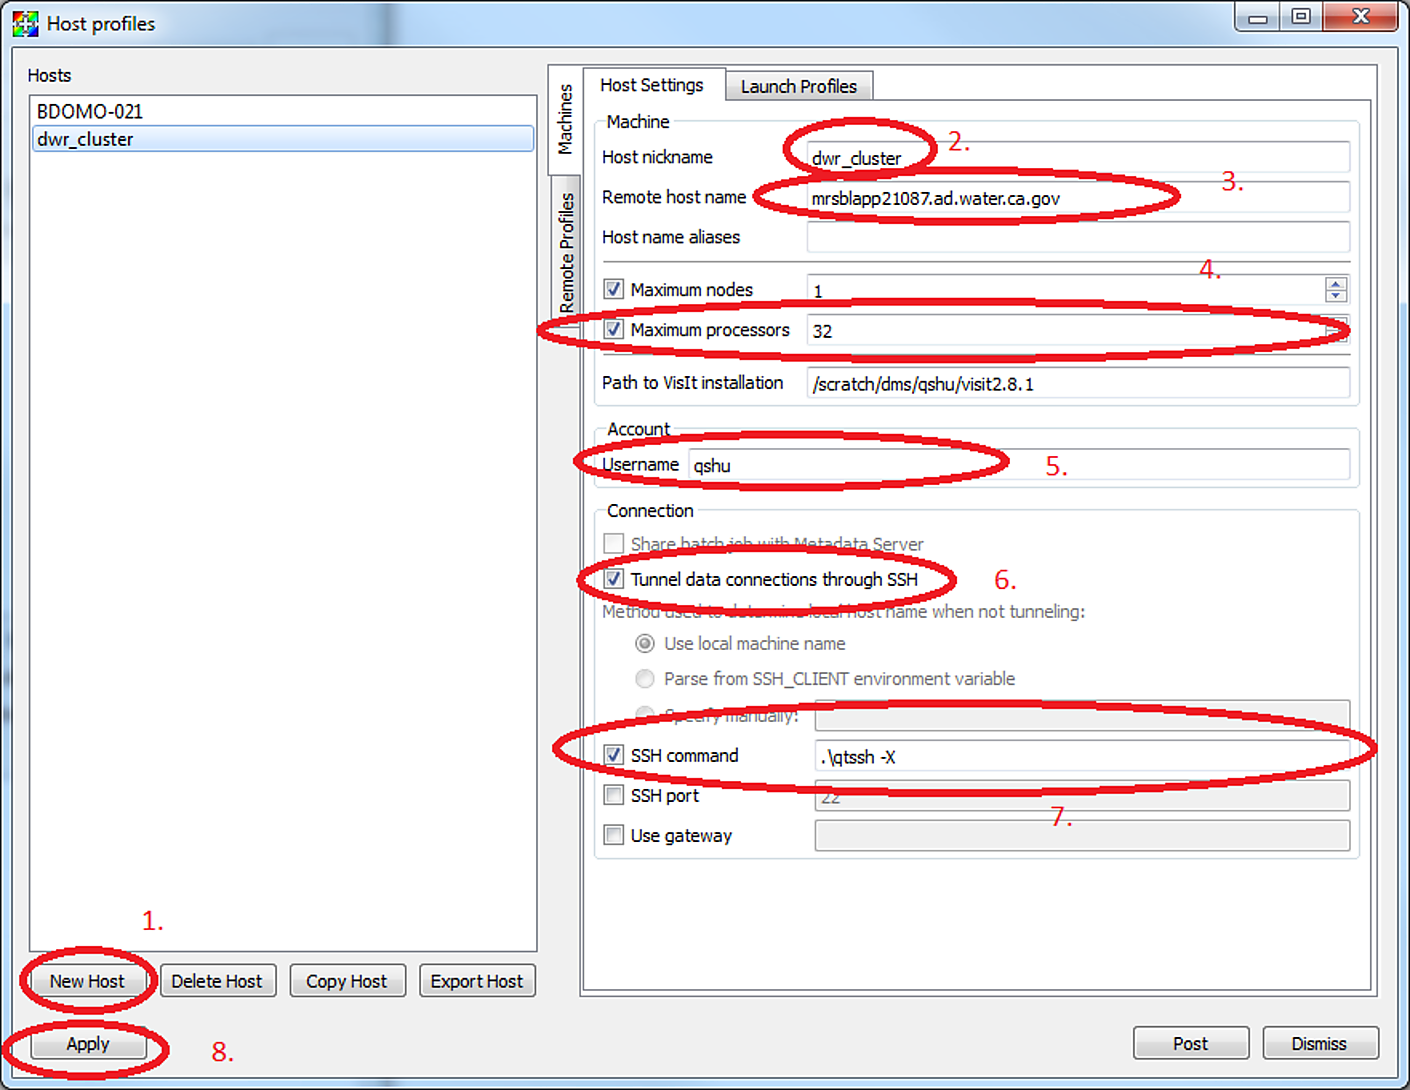
\includegraphics{setHostProfile}
        \caption{Creating a host profile}
        \label{figure:setHostProfile}
        \end{center}
        \end{figure}

On the host profile configuration window, you can can set up a  new host configuration by clicking button {\bf New Host} as shown in Figure \ref{figure:setHostProfile}.  You will need to input {\bf Host nickname}, {\bf Remote host name}, {\bf Maximum processors} and {\bf Username }. For the host shown in the figure, the VisIt installation path is already on the user's path environment and there is no need to specify the directory. If the VisIt path is not added into the bash search path, you would need to specify it in the box  {\bf Path to VisIt installation}.  Select {\bf ssh tunneling} under {\bf Connection}. To apply the configuration, click {\bf Apply}. To save the host settings for later, you need to save host settings using {\bf Options \textrightarrow Save Settings}.


If the host supports parallel processing, a user can save a parallel launch profile for the host as shown in Figure \ref{figure:setHostProfileParallel1}. Check the radio button {\bf Launch parallel engine} to activate the remote VisIt parallel engine as shown by Figure \ref{figure:setHostProfileParallel2}.   

        \begin{figure}
        \begin{center}
        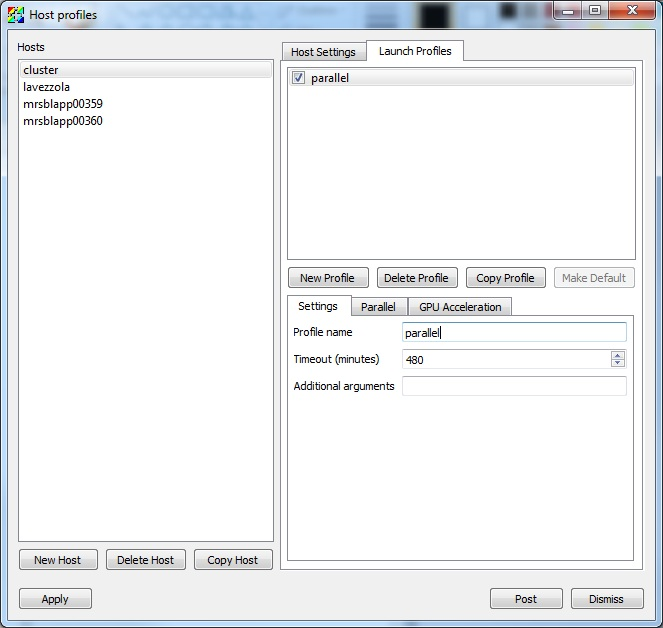
\includegraphics{setHostProfileParallel1}
        \caption{Set parallel profile}
        \label{figure:setHostProfileParallel1}
        \end{center}
        \end{figure}


        \begin{figure}
        \begin{center}
        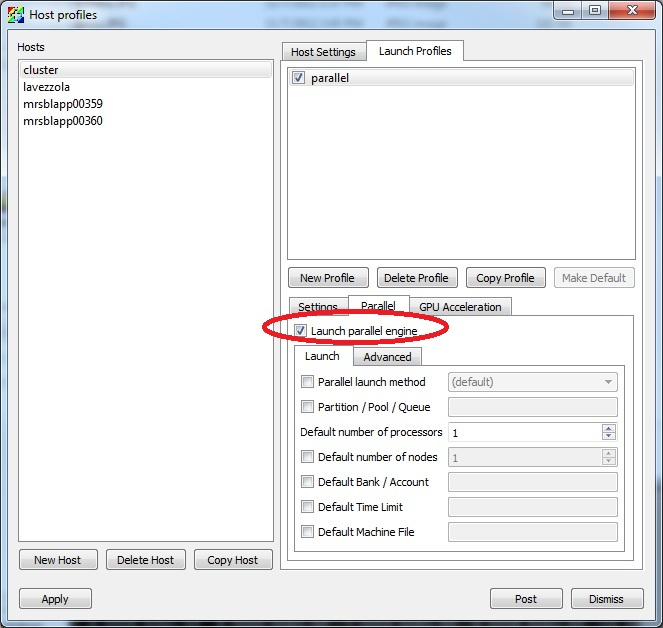
\includegraphics{setHostProfileParallel2}
        \caption{Activate parallel engine}
        \label{figure:setHostProfileParallel2}
        \end{center}
        \end{figure}


   Possible problem in setting up Server client mode:

   \begin{itemize}

    \item Symptom: VisIt completes some steps of the connection, including authentication with the remove server by ssh. However the console window appears and disappears immediately. VisIt then stops and keeps waiting for a reply from remote server as shown in the Figure \ref{figure:failToStart}.

        \begin{figure}
        \begin{center}
        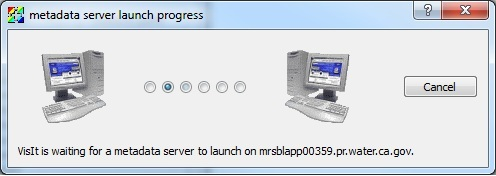
\includegraphics{failToStart}
        \caption{Error: Failing to start the remote VisIt engine}
        \label{figure:failToStart}
        \end{center}
        \end{figure}

Possible solution: This can happen because the compiled VisIt depends on gcc-4.3.5 or higher. GCC is the native compiler 
used by Linux, but some systems have older versions lurking in the background and if VisIt was compiled expecting runtime
features from a newer version it can fail. To check on this, you may need to examine the default GCC version loaded by your
bash\_profile. This is a configuration that is read in and executed every time you log in to Linux (even remotely). 
If you are using the DWR cluster mrsblapp20814, check your {\bf .bashrc} file to make sure the file {\bf /usr/local/dms/bashrc} is sourced. 

Then create a {\bf .bash\_profile} under your home directory and add following lines into it:\\

\begin{verbatim}
if [ -f ~/.bashrc ]; then\\
      . ~/.bashrc\\
fi\\
\end{verbatim} 
\end{itemize}

   
\chapter{Using the Plugins}
 
 VisIt software is developed by Lawrence Livermore National Laboratory (LLNL) and is open source. On the webpage  \url{https://wci.llnl.gov/codes/visit/manuals.html} user can find comprehensive introduciton and manual for VisIt user interface. \url{http://www.visitusers.org} provides many advanced topics about VisIt programming. 

\section{Opening Files}
To open a binary file for the first time, start VisIt and select {\bf Open \textrightarrow File}. 
When the file chooser appears, toggle the {\bf the Open file as type} option 
to the type of file you want to open (\emph{SCHISM}, \emph{gr3}, \emph{prop})
as shown in the red rectangle in the Figure \ref{figure:openFile}. 
Omitting the file choice is the most frequent source of problems. If these file types do 
not appear at all it may indicate a problem with the plugin installation.
 
\begin{figure}
\begin{center}
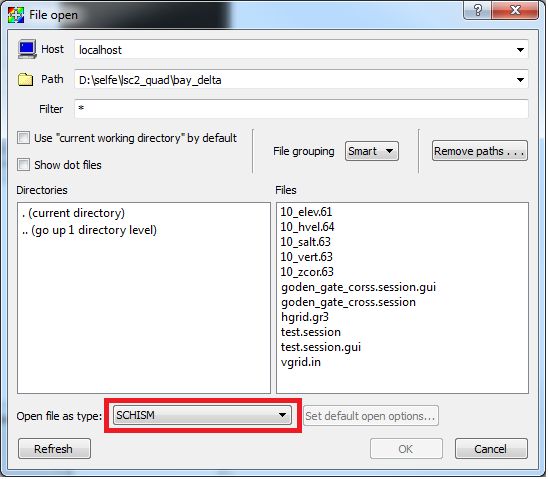
\includegraphics{visitOpenFile}
\caption{Opening a file in SCHISM format}
\label{figure:openFile}
\end{center}
\end{figure}

To view a SCHISM element-centered data file (for instance, extension .66 or .prop) you must have 
an \emph{hgrid.gr3} file located in the same directory.  This file defines the 2D horizontal 
unstructured mesh upon which the element-centered data are defined. 
To open a SCHISM gr3 or prop files, you need to set {\bf the Open file as type} option to \emph{gr3} or \emph{prop} rather than {\emph SCHISM}.

Adding the SCHISM file to preferred database plugins will avoid unnecessary failures during some complex VisIt operations with SCHISM files. This preference can be set using the {\bf Options \textrightarrow Plugin manager} 
option from the main interface, as shown in Figure \ref{figure:preferDatabase}.
	
        \begin{figure}
				\begin{center}
        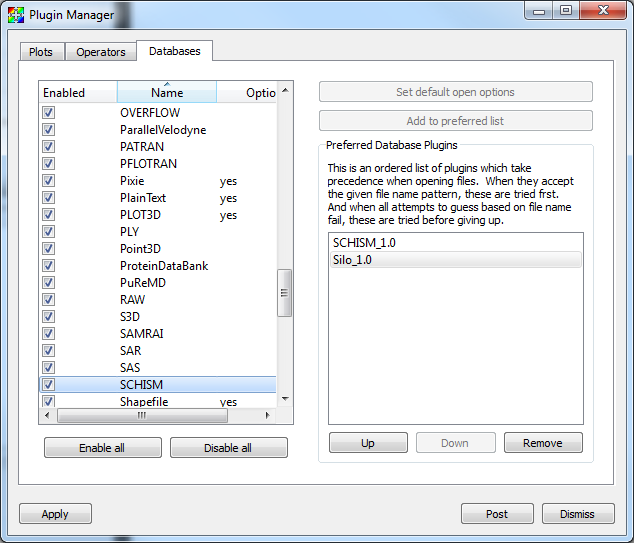
\includegraphics{preferDatabase}
        \caption{Adding SCHISM as the preferred database type}
        \label{figure:preferDatabase}
        \end{center}
        \end{figure}
				
We have came cross a problem that the button {\bf Add to preferred list} greyed out when user selected plugin \emph{SCHISM}. As the understanding of the source code review, VisIt don't allow the first loaded plugin to be added to preferred list. In such a case it
is most probably that \emph{SCHISM} is loaded before all the other plugins in the VisIt initialization. User can check the order of
loading in the mdserver log file after starting VisIt in debug mode.  A fix for this issue is to move the \emph{SCHISM} plugin dlls
from user home directory to \url {/VisIt/_install/_path/databases}. 
				
\subsection{Open vs Reopen vs Refresh}
A common question for new VisIt users is what the difference is between {\bf Open}, {\bf Refresh} and {\bf Reopen}.
To understand this, it is helpful to realize that VisIt can cache a lot of the data it has opened. This can
make panning through time faster the second time than the first. {\bf Refresh} will cause a file to be reloaded,
applying the plot settings to the new data. {\bf Reopen} is more commonly used on time grouping files (we'll cover these
in section \ref{sec:time}.
        
 \section{Displaying the Mesh}
You can view the mesh from the binary file by clicking the {\bf Add} button on the {\bf Plots} panel. Select {\bf Mesh} 
in the submenu, which should give you five options: {\bf 2D\_Mesh}, {\bf 3D\_Mesh} ,{\bf Layer\_Mesh},{\bf side\_center\_2D} and
{\bf side\_center\_3D}, choose one of them.
(Figure \ref{figure:meshItems}).  
        \begin{figure}
        \begin{center}
        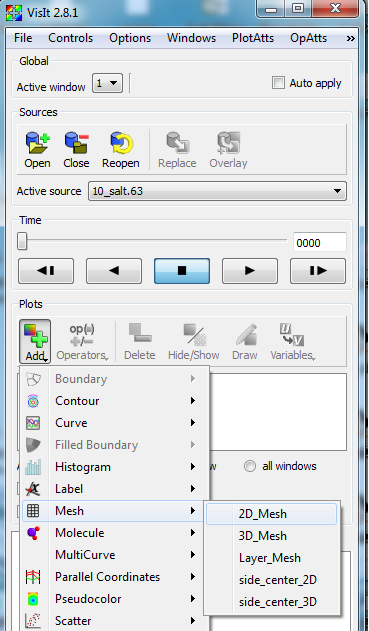
\includegraphics{meshItems}
        \caption{Mesh plots}
        \label{figure:meshItems}
        \end{center}
        \end{figure}
				
The table \ref{tab:meshComments} summarize some import features of those five options and  the {\bf SCHISM} output
defined over those mesh or point group.

\begin{table}
	\centering
		\begin{tabular}{|l|c|c|c|r|}
\hline
Name            & Dimension & Basic Element              &  Topology & Example \\
\hline \hline
2D\_Mesh        & 2D        & Triangle and Quadrilateral & 2D        & elev.61,wind.62,dtbe.66 \\
3D\_Mesh        & 3D        & Prism                      & 3D        & salt.63,hvel.64,salt.70 \\
Layer\_Mesh     & 3D        & Triangle and Quadrilateral & 2D        & vert.69 \\
side\_center\_2D& 2D        & 2D\_Mesh Edge Center       & NA        & NA\\
side\_center\_3D& 3D        & 3D\_Mesh Edge Center       & NA        & hvel.67\\
\hline
		\end{tabular}
	\caption{Unstructured meshes used in SCHSIM output.}
	\label{tab:meshComments}
\end{table}

   
At this point you have described the plot but not yet rendered it. Click the {\bf Draw } button on the {\bf Plots} panel 
to display the 3D  mesh as shown in Figure \ref{figure:mesh2}, you may wait a few seconds for the finished product. You can move, rotate and zoom in on the plot using mouse and keyboard.  

To better display the layered structure of the original mesh, you may need to exaggerate Z-dimension using visit transform operation. 
To apply a transform operation, first select the transform operation as shown in Figure \ref{figure:transform}. 
VisIt will apply a default transform operation on the plot, which initially may just lead to a empty plot. 
To create the desired transform, select the {\bf opAtts} on the main VisIt menu, then {\bf transform} and make the selection shown 
in Figure \ref{figure:transformPar}. A {\bf Transform operator attributes} window will pop up. Select the {\bf Scale}
option and change the scale value for {\bf Z} to a number bigger than 1, say 400 as shown in Figure \ref{figure:transformParSet}.
Click {\bf Apply} button to finish; you may need to click {\bf Draw} again to update the plot.
   
   
        \begin{figure}
        %\begin{center}
        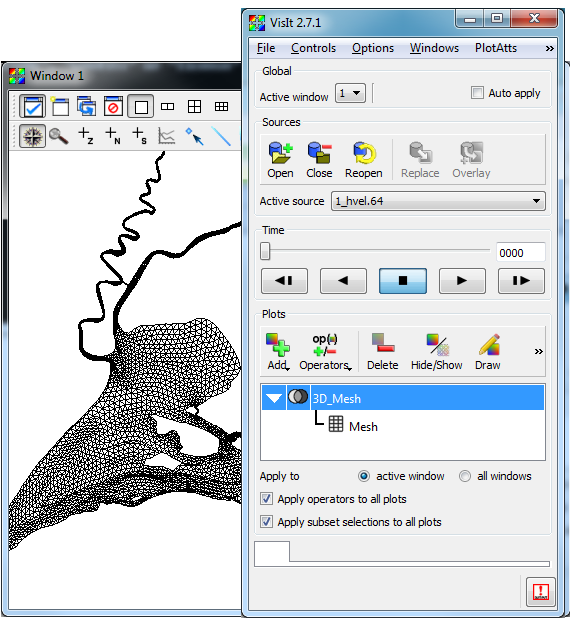
\includegraphics{mesh3D}
        \caption{3D mesh}
        \label{figure:mesh2}
        %\end{center}
        \end{figure}
       
       
        \begin{figure}
        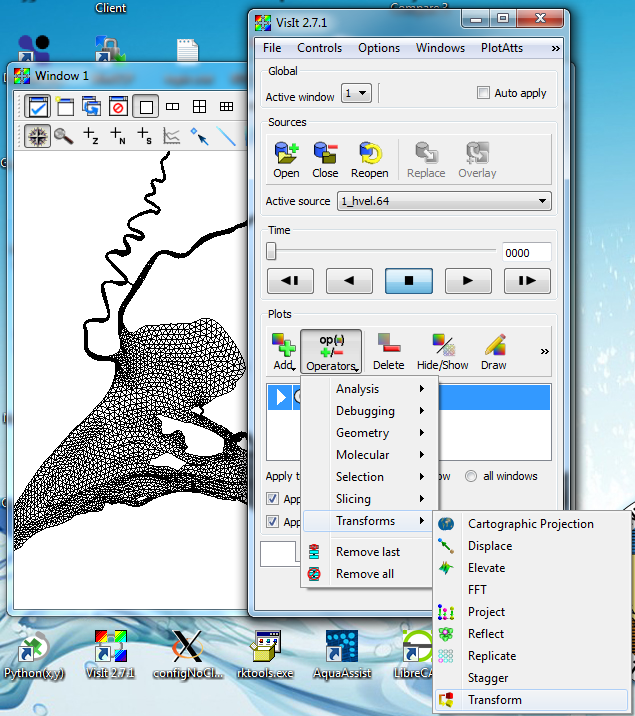
\includegraphics{transform}
        \caption{Transform operation}
        \label{figure:transform}
        \end{figure} 
   
   
        \begin{figure}
        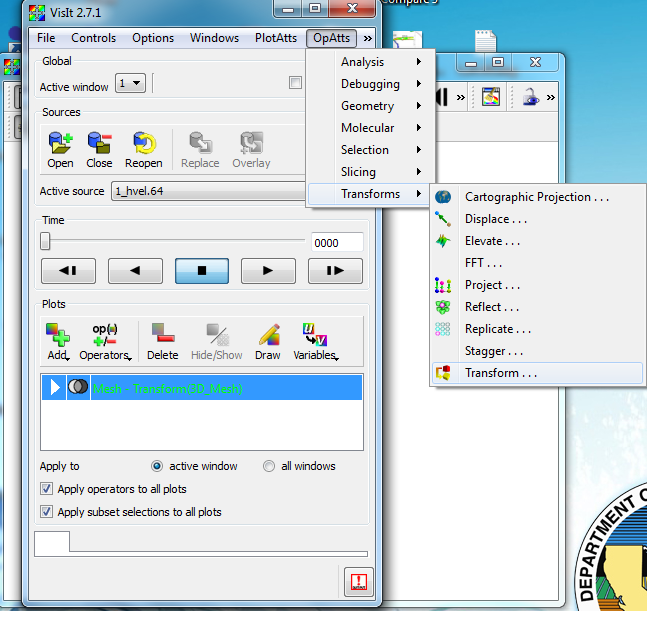
\includegraphics{transformPar}
        \caption{Transform menu}
        \label{figure:transformPar}
        \end{figure} 
      
        \begin{figure}
        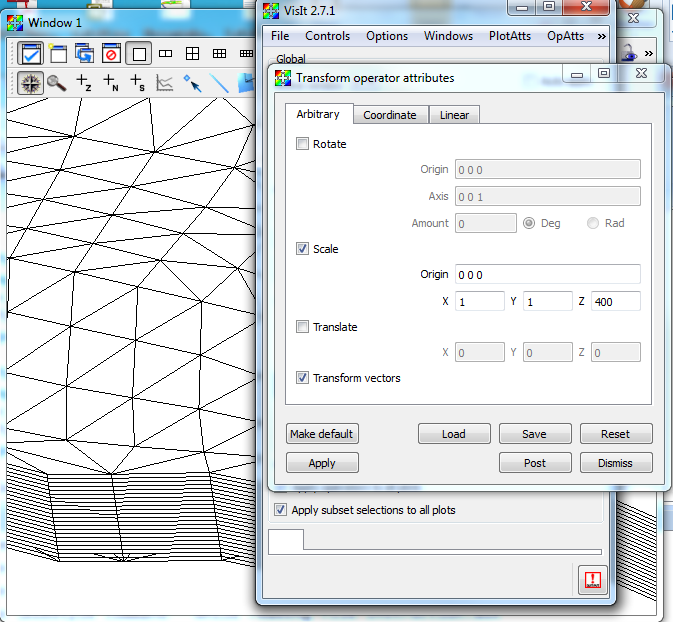
\includegraphics{transformParSet}
        \caption{Set transform parameters }
        \label{figure:transformParSet}
        \end{figure} 
        
  \section{Plotting Model Variables}\label{subsection:viewstate}
     VisIt will automatically search data files for the state variables contained in them that it can display. 
		 The available variables will depend on the file you opened, centerings of the data (node, element) 
		 and whether the data in the file are 2D or 3D mesh. For instance, depth and surface are defined only over the 2D mesh.
		 In contrast, velocity is a 3D variable; its native centering is element sides and whole levels, but 
		 in SCHISM standard output (hvel.64) it is interpolated to nodes. In 3D, VisIt will also report the state of surface layer, bottom layer and
     depth averaged and treat them as state defined over a single layer.
     
     VisIt provides a number of ways that may be useful to plot state variables. The most common choice for
		 scalars such as salinity, elevation or velocity magnitude is the pseudocolor plot, which is an image with different colors
		 representing different values. For a model state defined over the 3D mesh, the user has the option of plotting the 
		 original state in 3D, the state on the surface/bottom and depth averaged states as shown in Figure \ref{figure:states}.
     
        \begin{figure}
        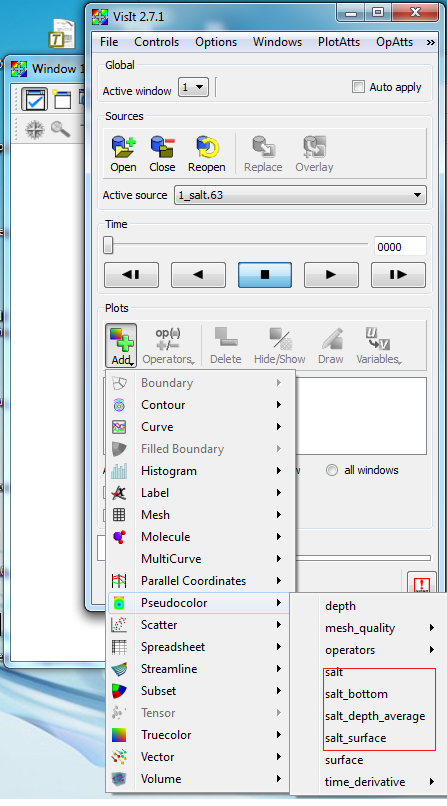
\includegraphics{states}
        \caption{Plots of model state variables }
        \label{figure:states}
        \end{figure} 
   
		 Figure \ref{figure:colorSalt} shows a pseudo color plot of surface salinity.
     
        \begin{figure}
        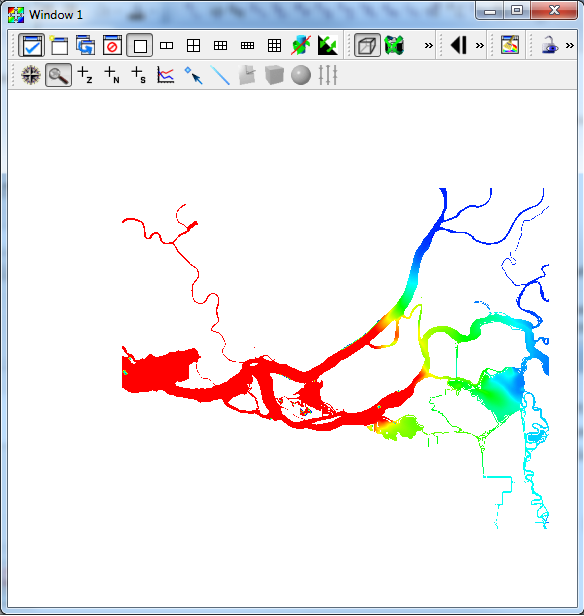
\includegraphics{colorPlot}
        \caption{Pseudocolor plot }
        \label{figure:colorSalt}
        \end{figure} 
				
			Another frequently used type is the vector plot, showing water velocity over the 2D or 3D grid. 
			This type of plot can be generated from SCHISM's hvel.64 output, 
			whose velocity vectors have been pre-interpolated to the nodes of model grid. Options are available to plot 
			depth averaged, surface or bottom velocity (which is usually very small).
      Figure \ref{figure:fractVelVector} shows a vector plot depth-averaged flow field at Fracts Tract in the Sacramento-San Joaquin
			Delta with a pseudo-color plot of velocity magnitude.

        \begin{figure}
        \begin{center}
        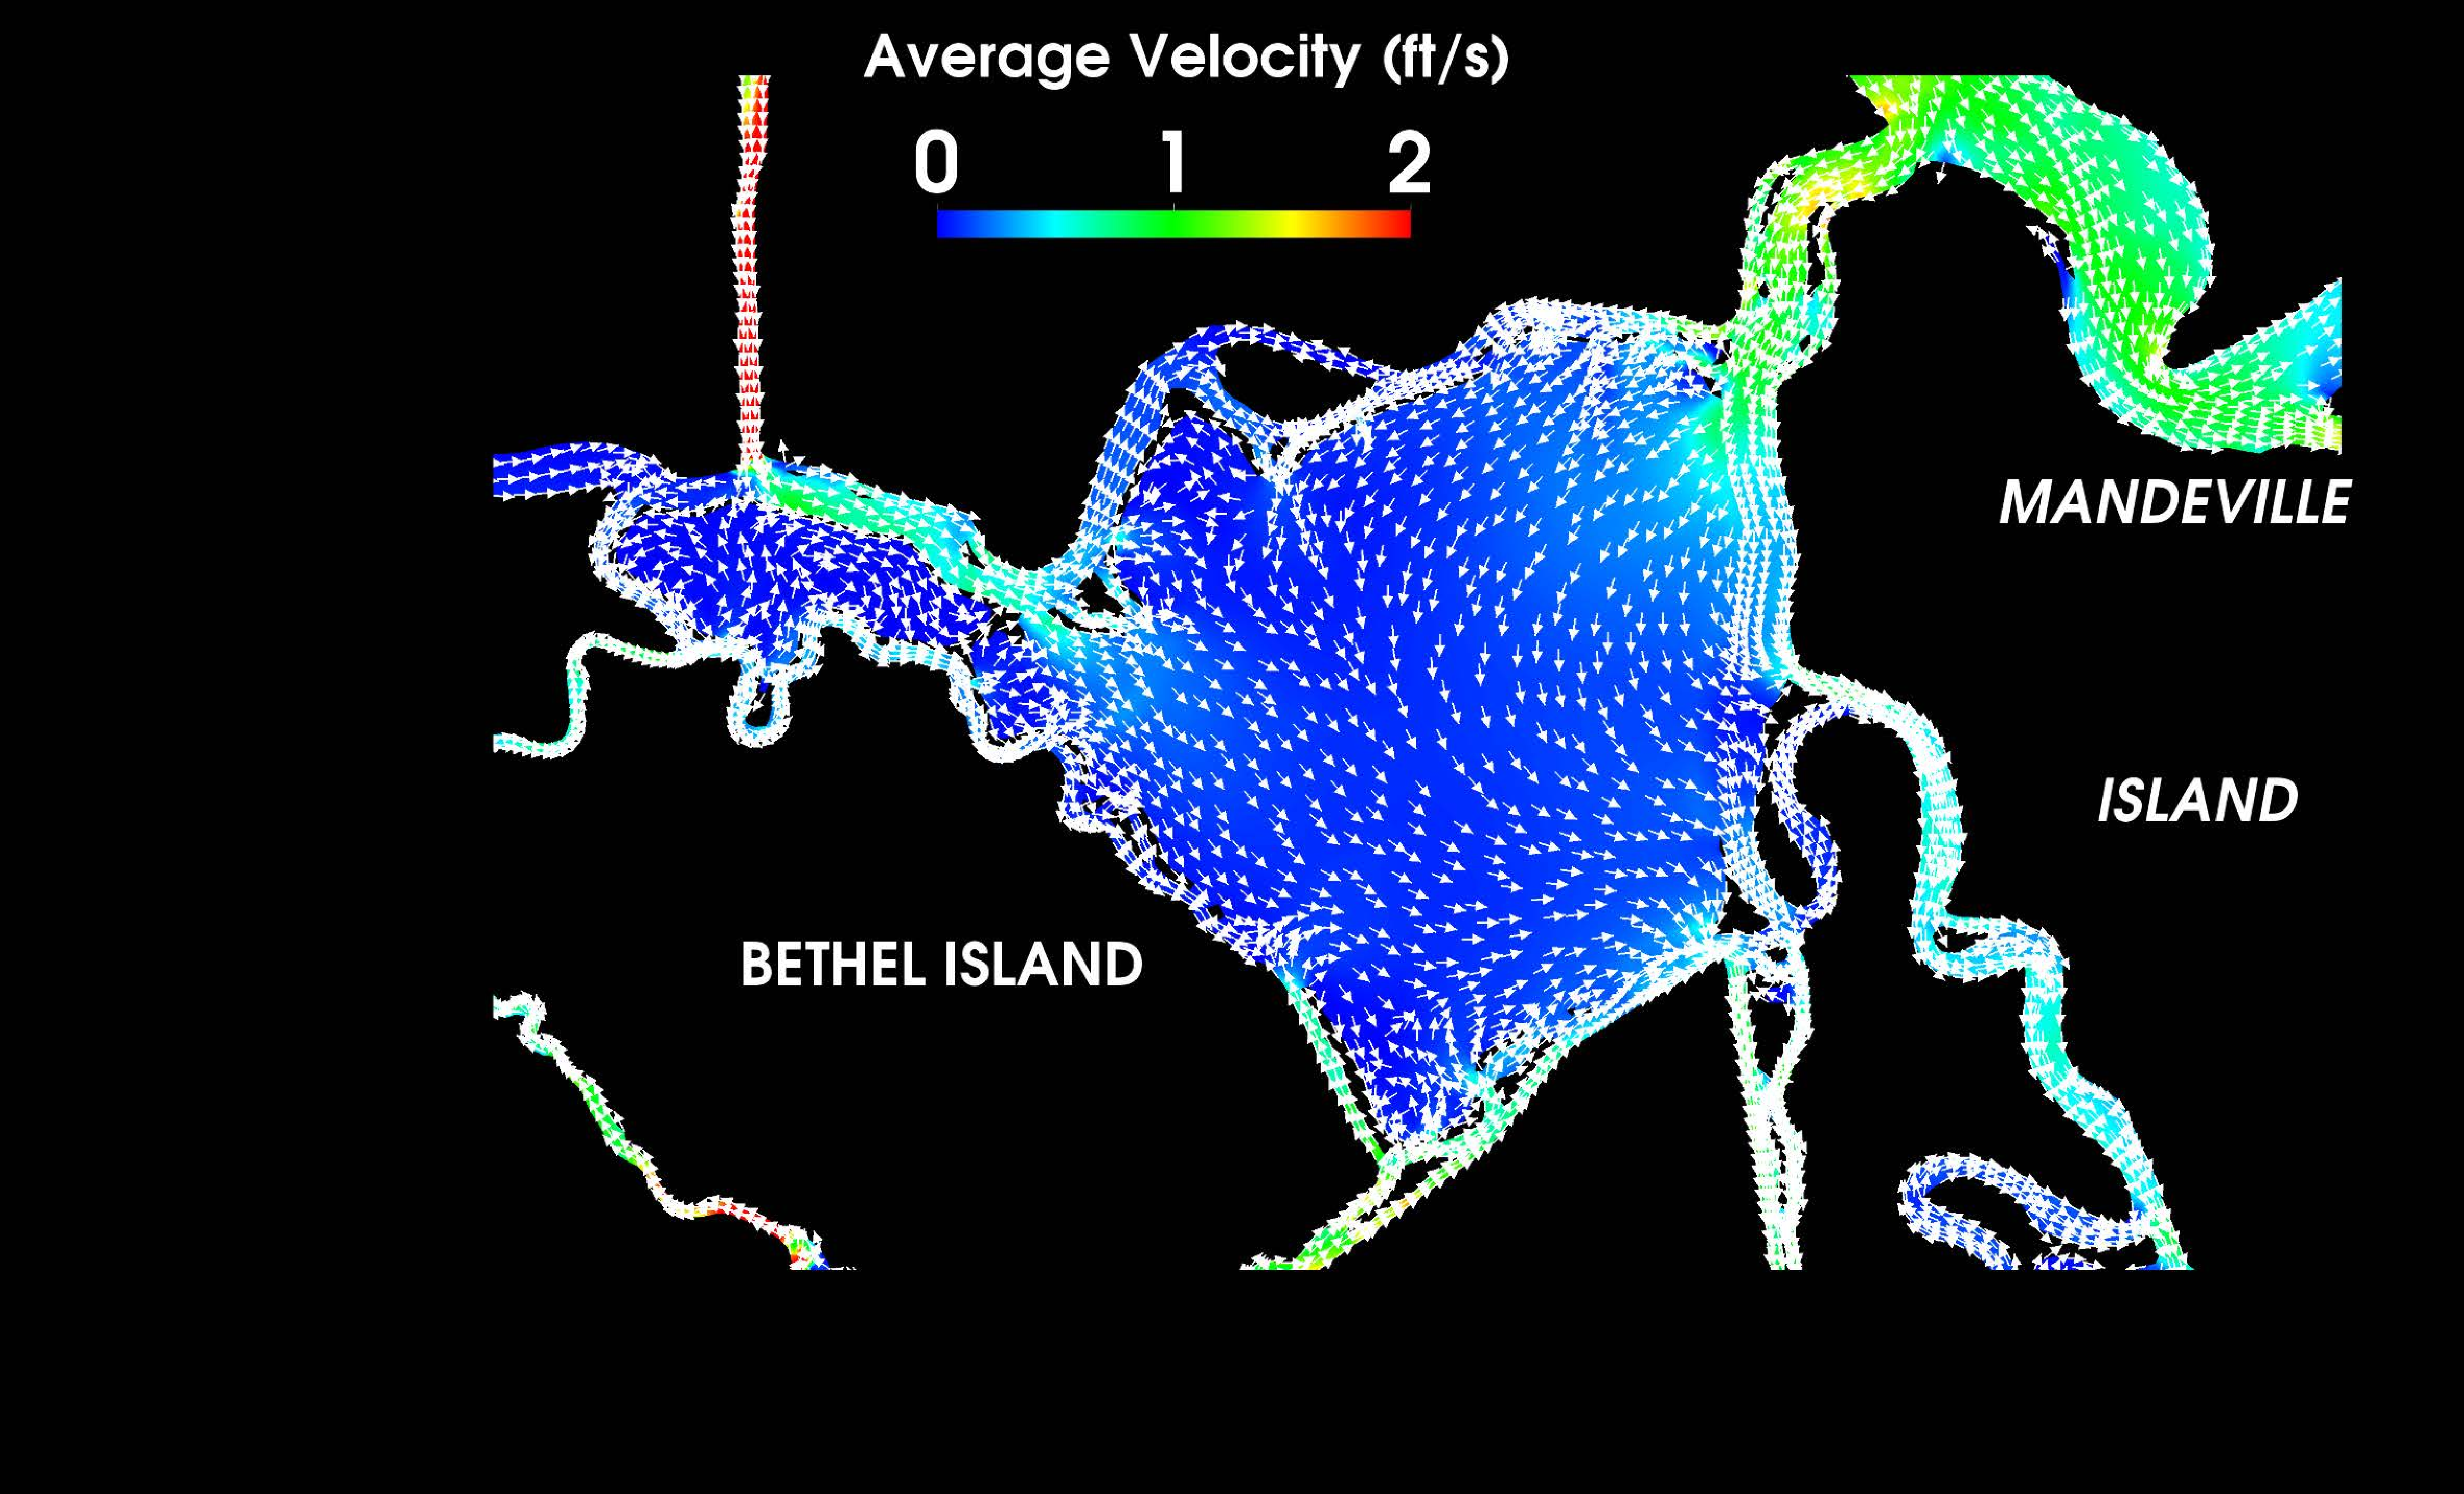
\includegraphics[scale=0.2]{fractVelVector}
        \caption{Velocity vector plot }
        \label{figure:fractVelVector}
        \end{center}
        \end{figure} 

A number of vector plot attribute need to be adjusted to get Figure \ref{figure:fractVelVector}. 
You need to set the vector density, vector color and arrow size options for the plot. The interface is shown in Figures \ref{figure:vectorStrideSet},Figure \ref{figure:vectorColorSet} and Figure \ref{figure:vectorGlyphSet}. 

Although you can show velocity magnitude using the size or color of the arrow glyphs, we have had more luck
rendering the arrows in a single color and size, with a background pseudocolor plot showing velocity magnitude.
In this case you need to add the pseudocolor plots; attributes are shown in Figure \ref{figure:vectorMagColorSet}
	    
			  \begin{figure}
        \begin{center}
        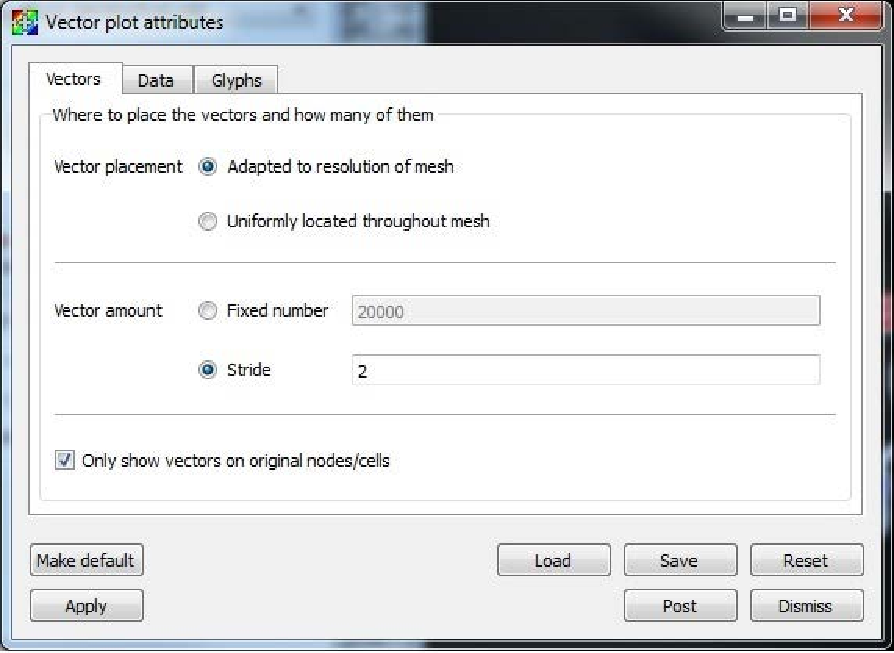
\includegraphics{vectorStrideSet}
        \caption{Setting vector density }
        \label{figure:vectorStrideSet}
        \end{center}
        \end{figure} 
				
				\begin{figure}
        \begin{center}
        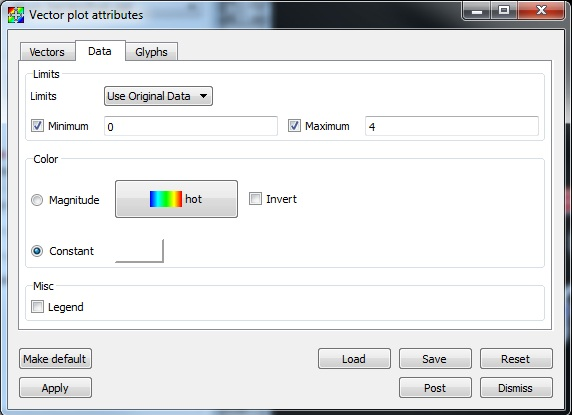
\includegraphics{vectorColorSet}
        \caption{Setting vector color }
        \label{figure:vectorColorSet}
        \end{center}
        \end{figure} 
				
				 \begin{figure}
        \begin{center}
        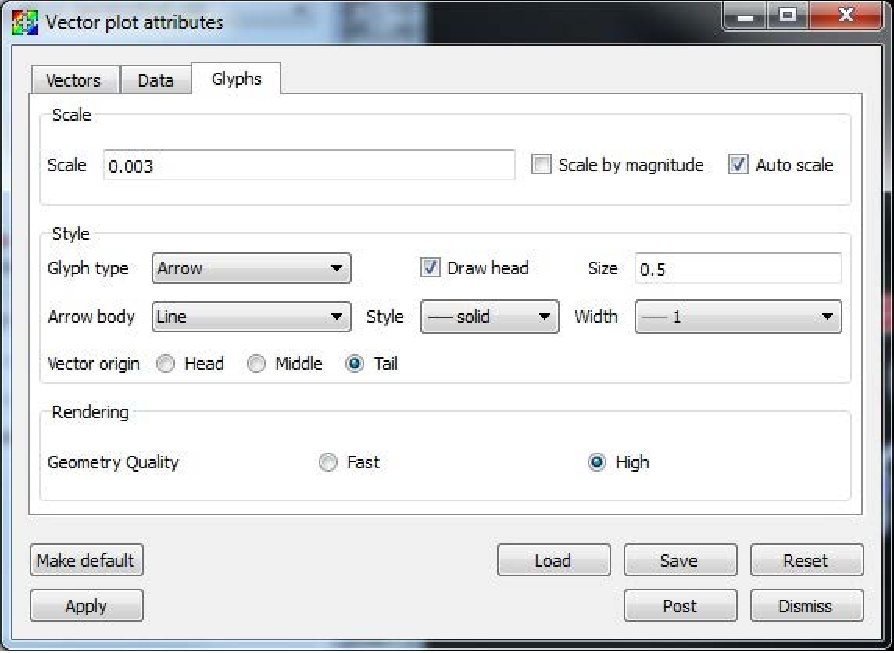
\includegraphics{vectorGlyphSet}
        \caption{Setting vector arrow }
        \label{figure:vectorGlyphSet}
        \end{center}
        \end{figure} 
				
					
				 \begin{figure}
        \begin{center}
        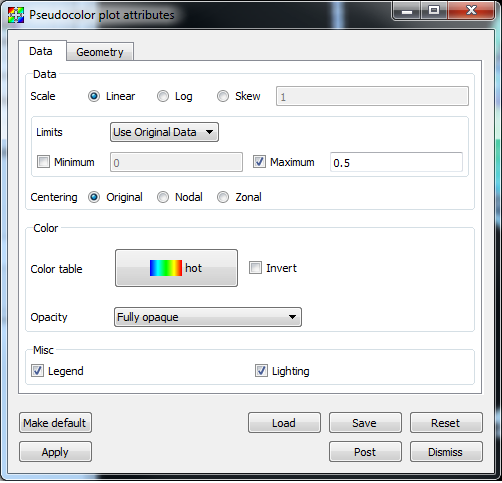
\includegraphics{vectorMagColorSet}
        \caption{Setting vector magnitude pesudocolor plot attributes }
        \label{figure:vectorMagColorSet}
        \end{center}
        \end{figure} 
				

\section{Time Sequence and File Grouping}
\label{sec:time}
Each SCHISM output data file contains a number of time steps -- for instance daily blocks of data saved once per hour are common.
Frequently, you will want to pan through time over more than one of these files, either to produce an animation
or to manually page through time manually. VisIt understand the time blocking concept; however, you must provide it
with information on the order of files. One mechanism that is available in VisIT that we will not cover is the virtual database.
A second option is to generate a simple .visit database grouping file to specify the order in which the files are encountered. Below is an example of \emph{.visit} file for salinity binary outputs:

\begin{verbatim}
====== File salinity.visit =======
		   200_salt.63
       201_salt.63
       202_salt.63
			  ... 
       215_salt.63
       216_salt.63
====== End of file ====
\end{verbatim}
				
After creating \emph{.visit} file, you can open it as SCHISM format file as shown in Figure \ref{figure:openFile}. After open the file, Visit will automatically check all the output files, counting total number of time step available. After counting is done, user should see a time slide control available on the Visit main interface as shown in Figure \ref{figure:timeVCR}.

You can correlate two or more grouping file with same time period together and to see the evolution of different state variable from different SCHISM output files.  For instance, you can over lay flow vector plot over a salinity background.  Say, you now have two group files, \emph{salt.visit} for salinity and \emph{hvel.visit} for flow field. Here is the steps of correlating two files:
\begin{enumerate}
\item Open \emph{salt.visit}.
\item Create \emph{Pesudocolor} plot of \emph{salt} and Draw it.
\item Open \emph{hvel.visit}.
\item Create \emph{Vector}  plot of \emph{horizontal\_velocity} and Draw it.
\item Open the {\bf Database Correlation} window from the {\bf Controls} menu.
\item Click the {\bf New...} button to generate a new database correlation using the {\bf Create database correlation} window.
\item Select both \emph{salt.visit} and \emph{hvel.visit} from the list and click the right arrow button to move
      them over into the list of {\bf Correlated sources}.
\item Select {\bf Time} for the {\bf Correlated method} so the time values from the databases are used to line up their time steps.
\item Click {\bf Create database correlation}. Note how the {\bf Active time slider} in the {\bf Time} controls is now set to the
      \emph{Correlation01} time slider. This new slider is used to control both \emph{salt.visit} and \emph{hvel.visit} plots.
\item Change the time state using the time slider in the {\bf Time} controls and watch both plots update.
\end{enumerate}



\section{Operators (GUI and Macro)}
VisIt operators can help you transform results: slicing, rotating, transforming or filtering. The possibilities
are covered pretty well in the VisIt documentation, so here we are going to discuss only a few options that we
use pretty often. One of them also provides an introduction to VisIt macro scripting.
    
    \subsection{Selection}\label{sec:thresholdOperator}
    
    The threshold operator is used to mask out out-of-bounds values. 
		The most common use of it is to mask out the dry elements in the domain. 
		For this purpose, you would use selection by threshold to remove the dryout cells. 
		Click {\bf Operators} on the {\bf plots} panel of the VisIt 
		main menu and select the {\bf Selection} menu item. A popup showing
    selection options will appear as in Figure \ref{figure:thresholdSelection}. 
		Select {\bf threshold}. Usually this operator will lead to
    a empty plot with default parameters and you will need set up your own and delete the default. 
		The example in Figure \ref{figure:colorSalt} is intended to admit
		only physically meaningful salinity, filtering 
		dry regions. Click {\bf OpAtts} on the top toolbar of the VisIt main menu 
		and choose {\bf Selection}. Then a popup submenu showing selection option will 
		show up as Figure \ref{figure:thresholdSelectionProp}, select {\bf threshold}. In the new pop window, 
		you will need to remove the default threshold variable and choose 
		the correct variable with desired threshold interval as demonstrated in Figure
    \ref{figure:thresholdSelectionPropSet} and choose option {\bf All in range} under column {\bf Show zone if}.
     
        \begin{figure}
        \begin{center}
        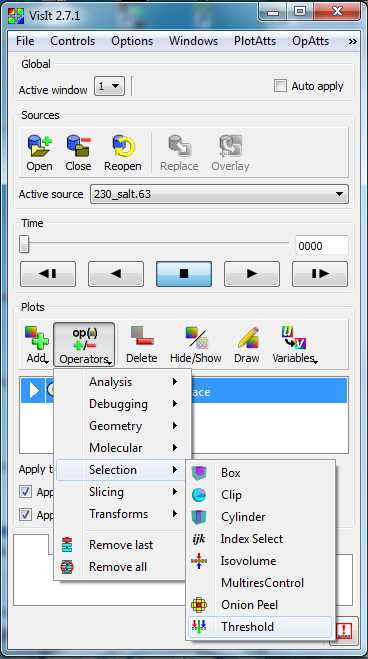
\includegraphics{thresholdSelection}
        \caption{Threshold selection }
        \label{figure:thresholdSelection}
        \end{center}
        \end{figure} 
        
        \begin{figure}
        \begin{center}
        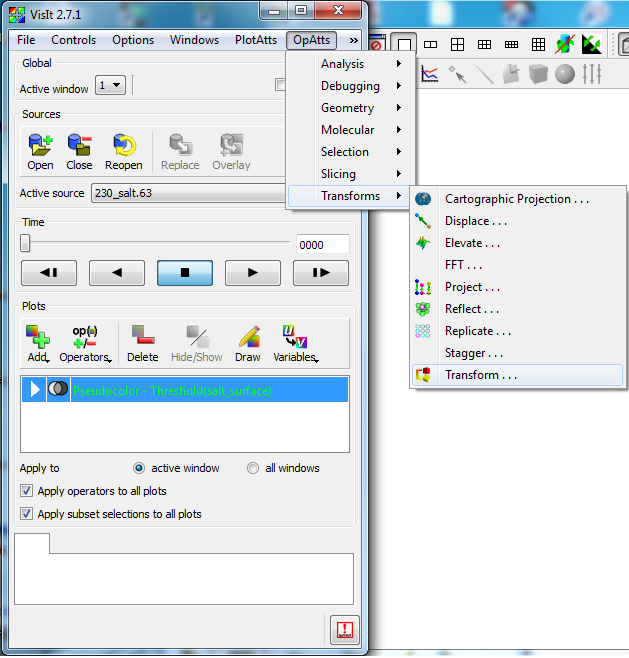
\includegraphics{thresholdSelectionProp}
        \caption{Threshold selection property }
        \label{figure:thresholdSelectionProp}
        \end{center}
        \end{figure} 
        
        \begin{figure}
        \begin{center}
        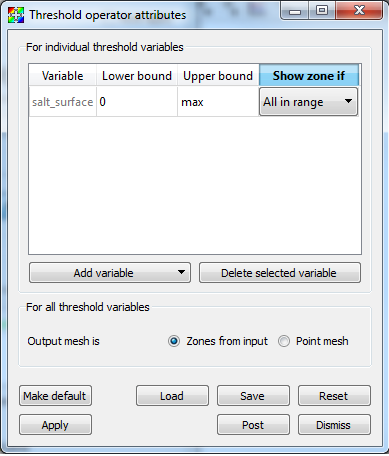
\includegraphics{thresholdSelectionPropSet}
        \caption{Threshold setting }
        \label{figure:thresholdSelectionPropSet}
        \end{center}
        \end{figure} 

	 \subsection{Cross-Section Slice (and Python Macro)}
	
	  The VisIt {\bf Slice} operator provides a 2D sliced view of the 3D data. 
		In this section, we use a VisIt Python Macro to define a set of plane points and normal vectors to create cutaway along a desired line. 
		
		Our example is a vertical profile of salinity running longitudinally along the Sacramento River 
		near Emmaton from SCHISM salinity output. The coordinates defining longitudinal transect section are
\begin{verbatim}
    (607899, 4.21483e+006),
    (610173, 4.21632e+006),
    (611124, 4.21716e+006),
    (612121, 4.2181e+006)
\end{verbatim}
			
    In addition, we will show three cross-stream sections running perpendicular to the main transect,
		defined by these segments:
\begin{verbatim}
				[(607706, 4.21508e+006),(608204, 4.21443e+006)],
				[(610080, 4.2163e+006),(610499, 4.21584e+006)],
				[(611180, 4.2173e+006),(612190, 4.2163e+006)].
\end{verbatim}
    
\subsubsection{Defining a Macro}
Our task will be performed by defining and running a Macro in VisIt. 
VisIt allows you to record your work using a Macro recorder, edit the result as a Python script
and then re-use the sequence of operations later at the push of a button. 
A lot of this is out of scope for this document and new users, but we think it is useful 
to know what to do if someone hands you some code.

To define the macro, select {\bf Controls \textrightarrow Commands}. In the popup windows, paste the code into a blank tab sheet.  Then click the {\bf Make macro} button at the bottom of the Window.  Visit will ask you give it a name. After done this step, go back to main interface, select {\bf Macros}. VisIt should provide you a window with a button for this Macro. The salt.63 file must be opened for Macro to work properly.		
		
		  \clearpage
		  %\begin{Code}
      %\centering
      \lstinputlisting[language=Python]{emmaton.py}
      %\end{Code}
				
      The resulting effect is shown in Figure \ref{figure:emmatonSalt3D}
			
			 \begin{figure}
       \begin{center}
       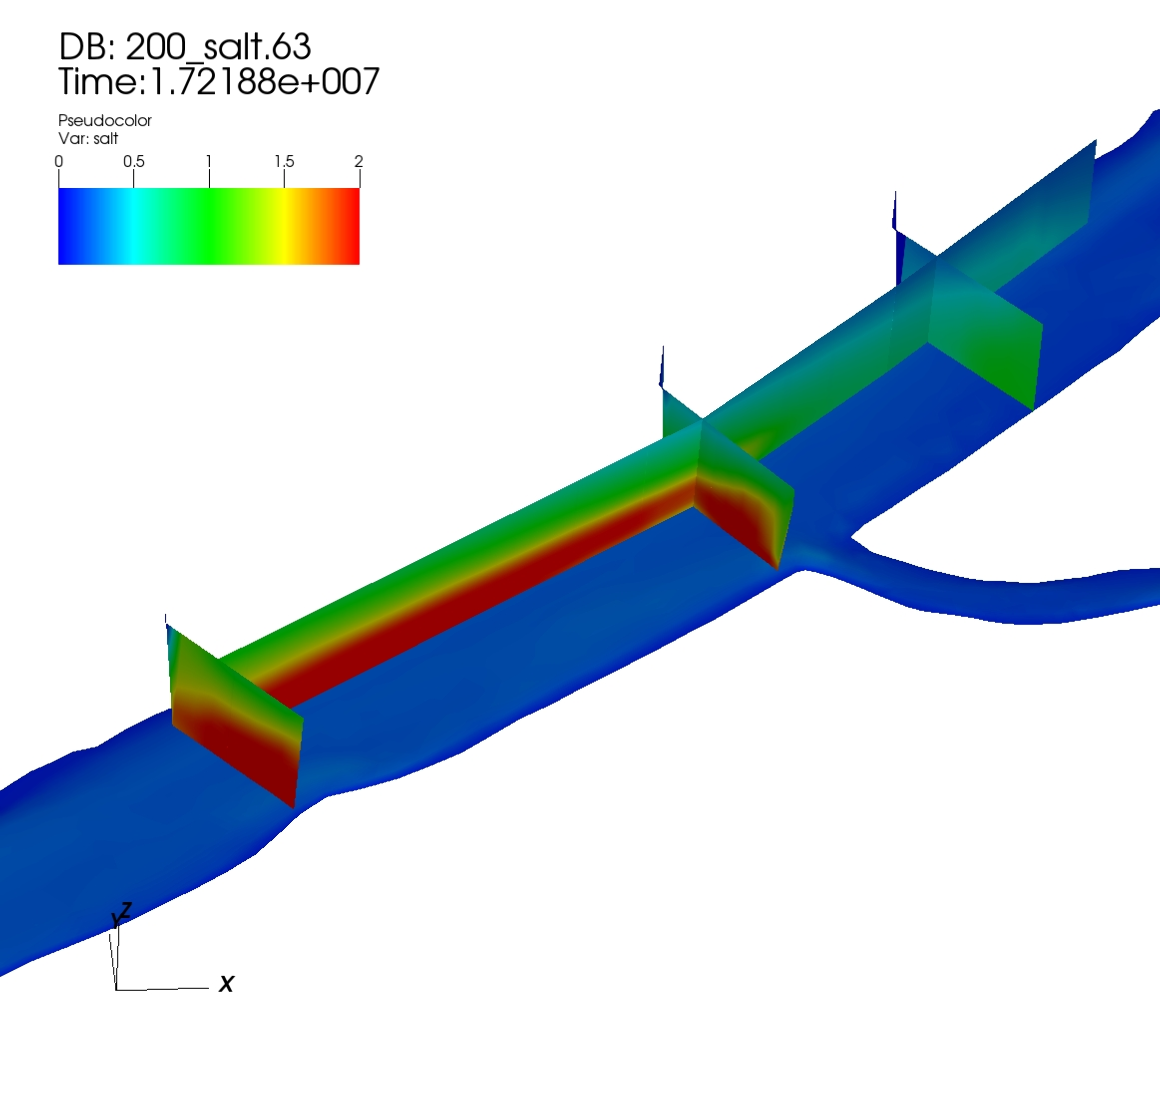
\includegraphics[height=100mm]{emmatonSalt3D}
       \caption{Salinity near Emmaton in Sacramento River }
       \label{figure:emmatonSalt3D}
       \end{center}
       \end{figure} 
			
	 \section{Image Quality}

Image quality for exported images is controlled via {\bf File \textrightarrow Set save options} 
from the main GUI menu. The settings will be applied only for saved still images. 
The term "`resolution"' is used, but what VisIt really allows you to do is set the image
size in pixels. This must be set to your desired image resolution multiplied by your intended
size. Figure \ref{figure:highQualityImageSet} shows a resolution of 4000x2424 for the image
plot of Figure \ref{figure:fractVelVector}. Although this may seem big, we have found that high
resolution is needed on plots with arrows. Furthermore, publications often require resolution
of 600dpi on raster plots.		
		 
\begin{figure}
\begin{center}
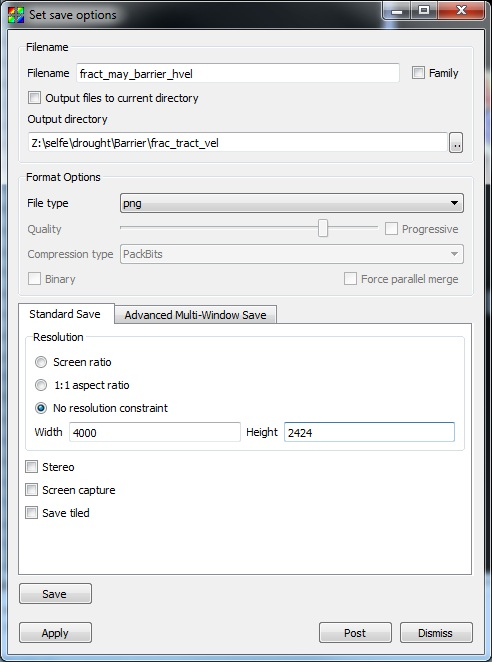
\includegraphics{highQualityImageSet}
\caption{Image output with high resolution }
\label{figure:highQualityImageSet}
\end{center}
\end{figure} 			

\section{VisIt Subsetting}

Besides the subsets defined by underlying mesh grid, VisIt provides powerful and customizable subsetting methods
to extract interested group based on combination of data values, defined expressions and operators. One interesting
usage of subsetting we found is to apply different plotting setup for a group of neighboring zones. 

Here is a image shows different  flow velocity vector density are desired at several water bodies, where each color
represents a water body.
\begin{figure}
\begin{center}
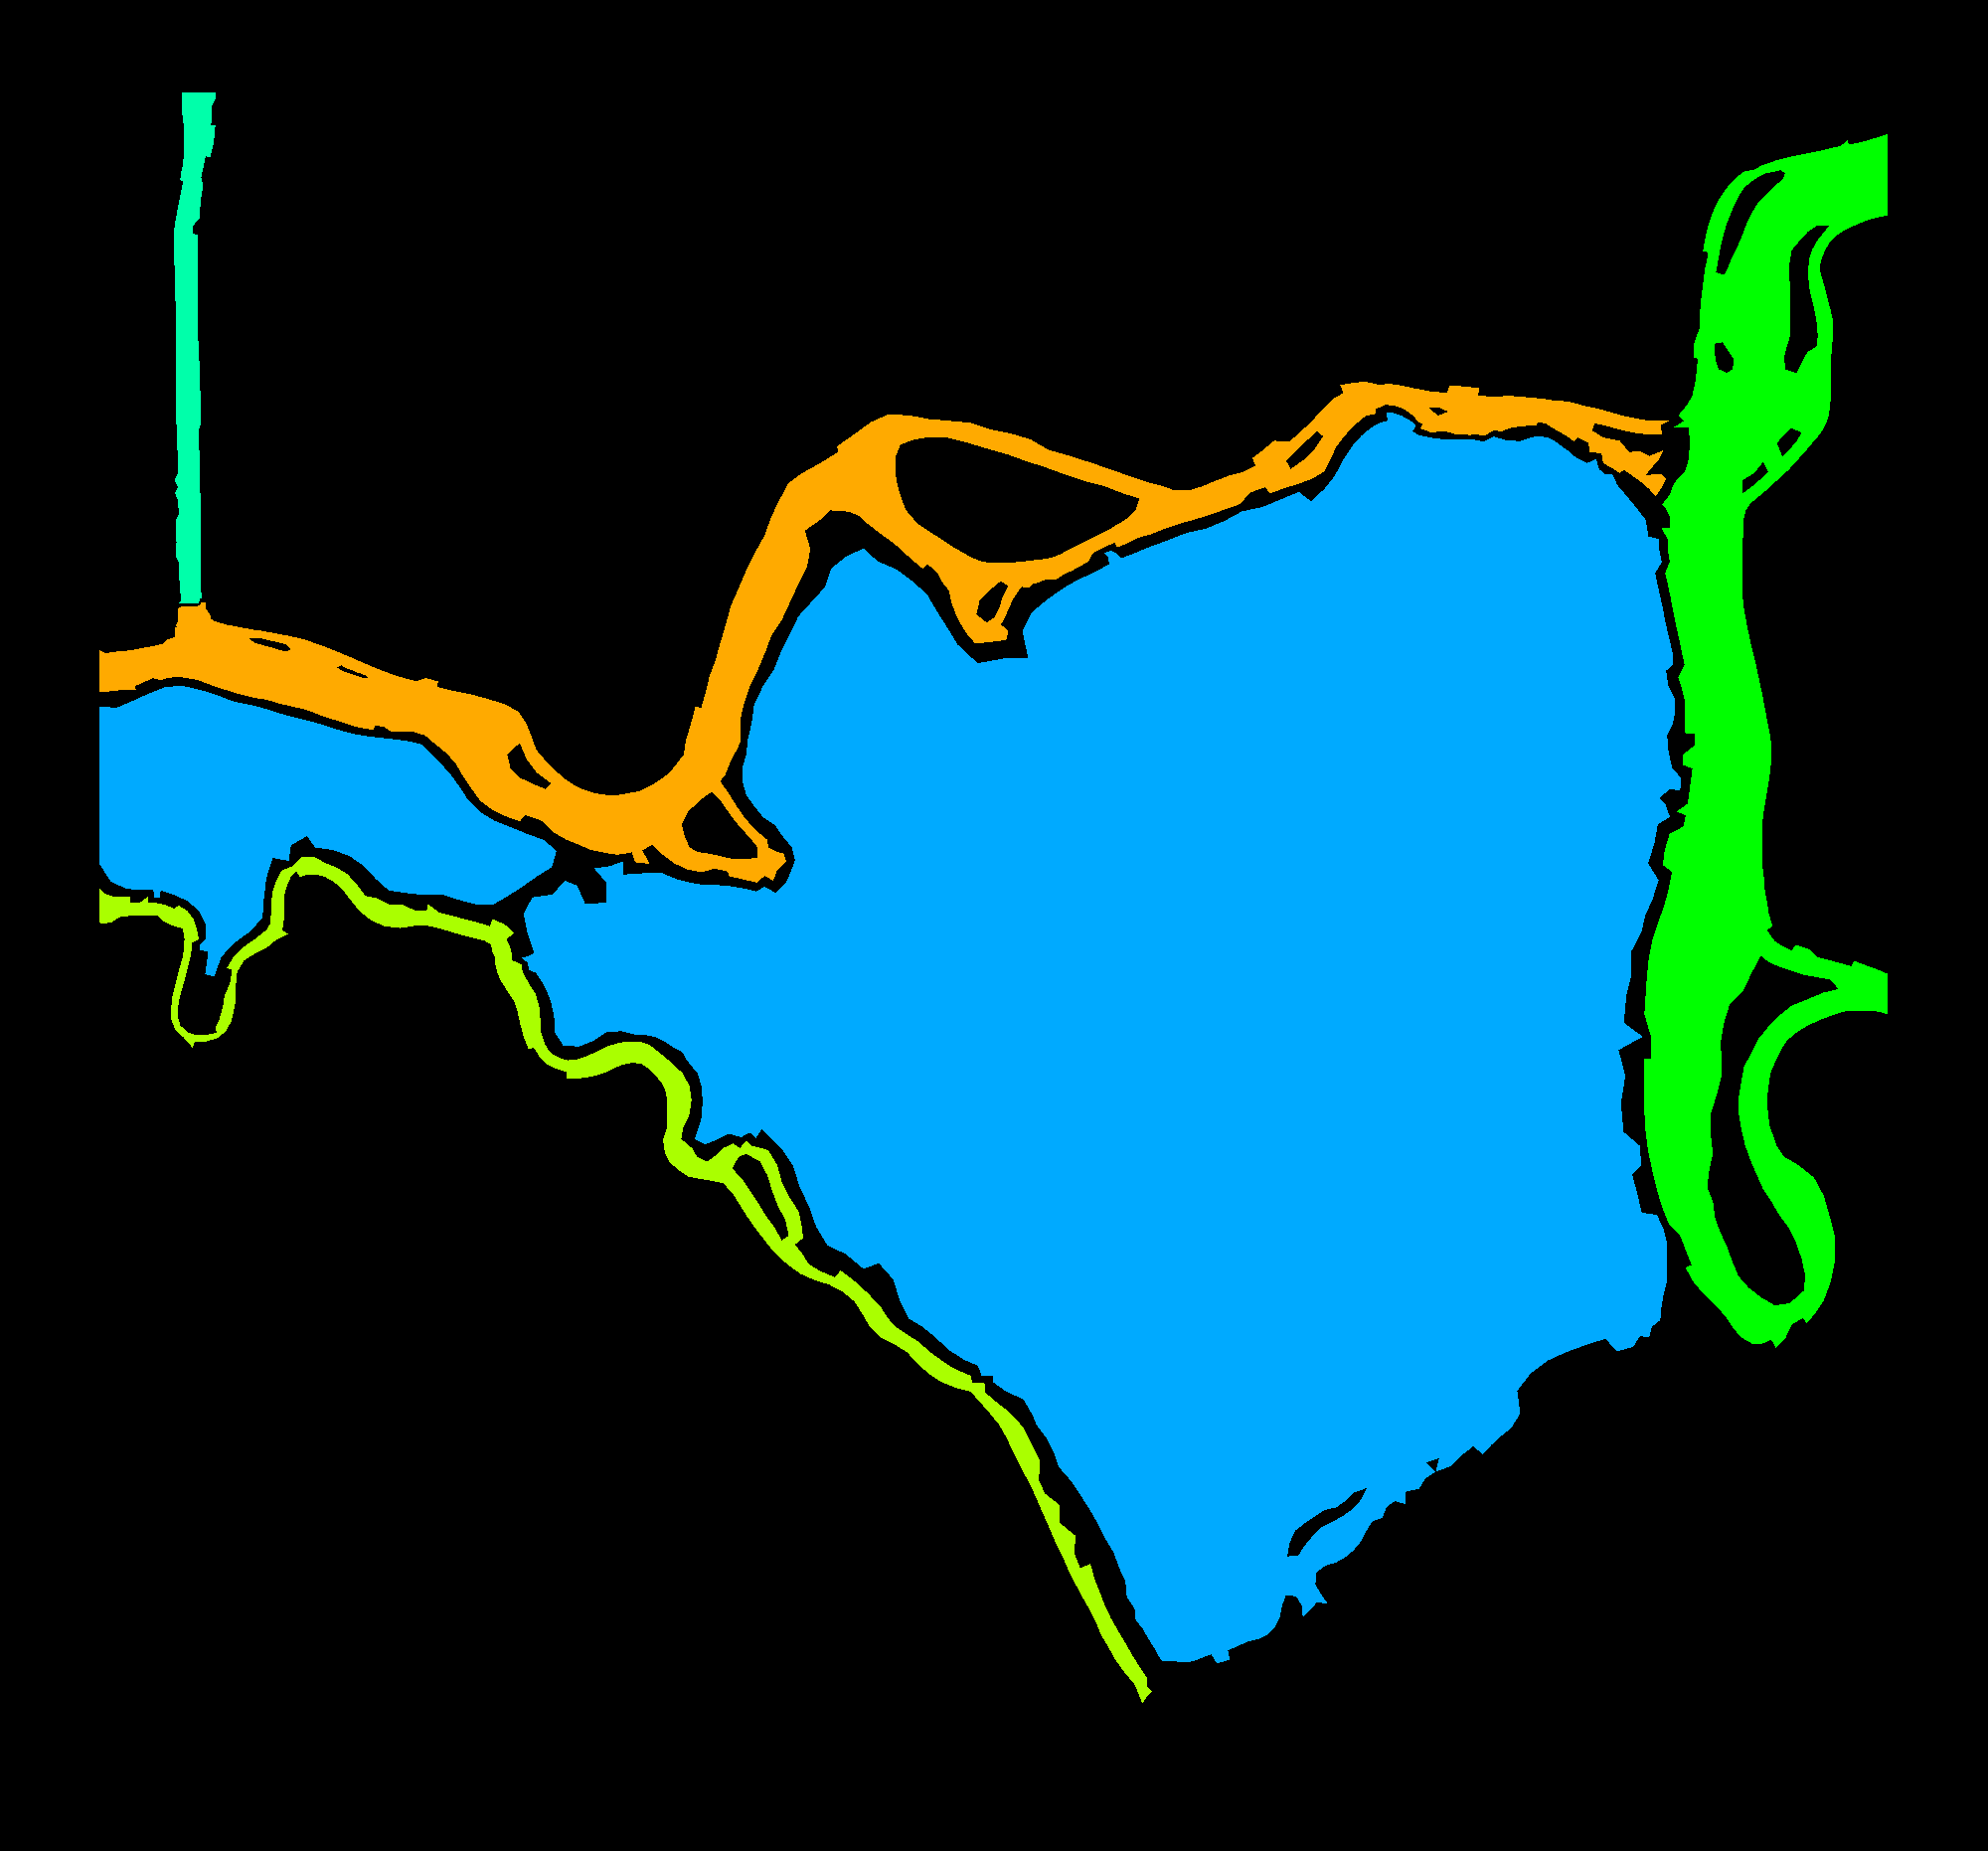
\includegraphics{franksTractZones600}
\caption{Water body delineation }
\label{figure:franksTractZones}
\end{center}
\end{figure} 	

VisIt enable user to extract the mesh points for each water body, save them as a named subsets and apply
the selected subsets to other type of plots. 

First of the all a raster grid is needed  to delineate water body. In
this example, we extracts the polygon points coordinates from a shape file with the help of ARCGIS tools. Then we convert
those polygons coordinates into a number of \emph{gr3} files in which all the mesh points inside a water body polygon are
flagged a nonzero identification integer.

To define a subsets in VisIt, first open the \emph{gr3} file. Given a example, the mesh points within the Franks Tract\
is defined by the \emph{gr3} file, {\bf mask\_franks\_tract.gr3}. The Frank Tracts is the blue zone in the figure \ref {figure:frankTractZones}. Then do a pseudo-color plot of the data value stored in {\bf mask\_franks\_tract.gr3}. The \emph{gr3}
file only store one type of value on each mesh node and the file name is used as the name of data value by default in VisIt.
Use \emph{Threshold} operations to filter out any points whose value is other than the identification integer of the Franks
Tract Zone as shown in the figure \ref{figure:franksTractZoneThreshold}, where the identifying integer of the Franks Tract is
1.


\begin{figure}
\begin{center}
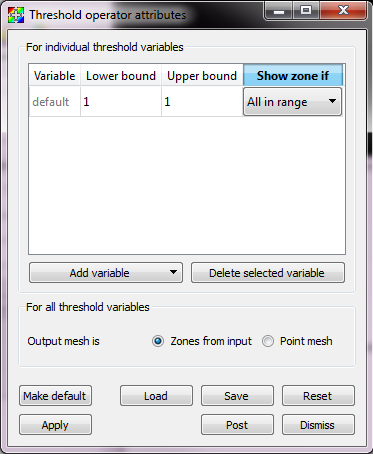
\includegraphics{franksTractZoneThreshold}
\caption{Water body threshold setting }
\label{figure:franksTractZoneThreshold}
\end{center}
\end{figure} 			

After applying the threshold operation on the pseudo-color plot, only the zone of Franks Tract will be left as the figure
\ref{figure:franksTractZone}.

\begin{figure}
\begin{center}
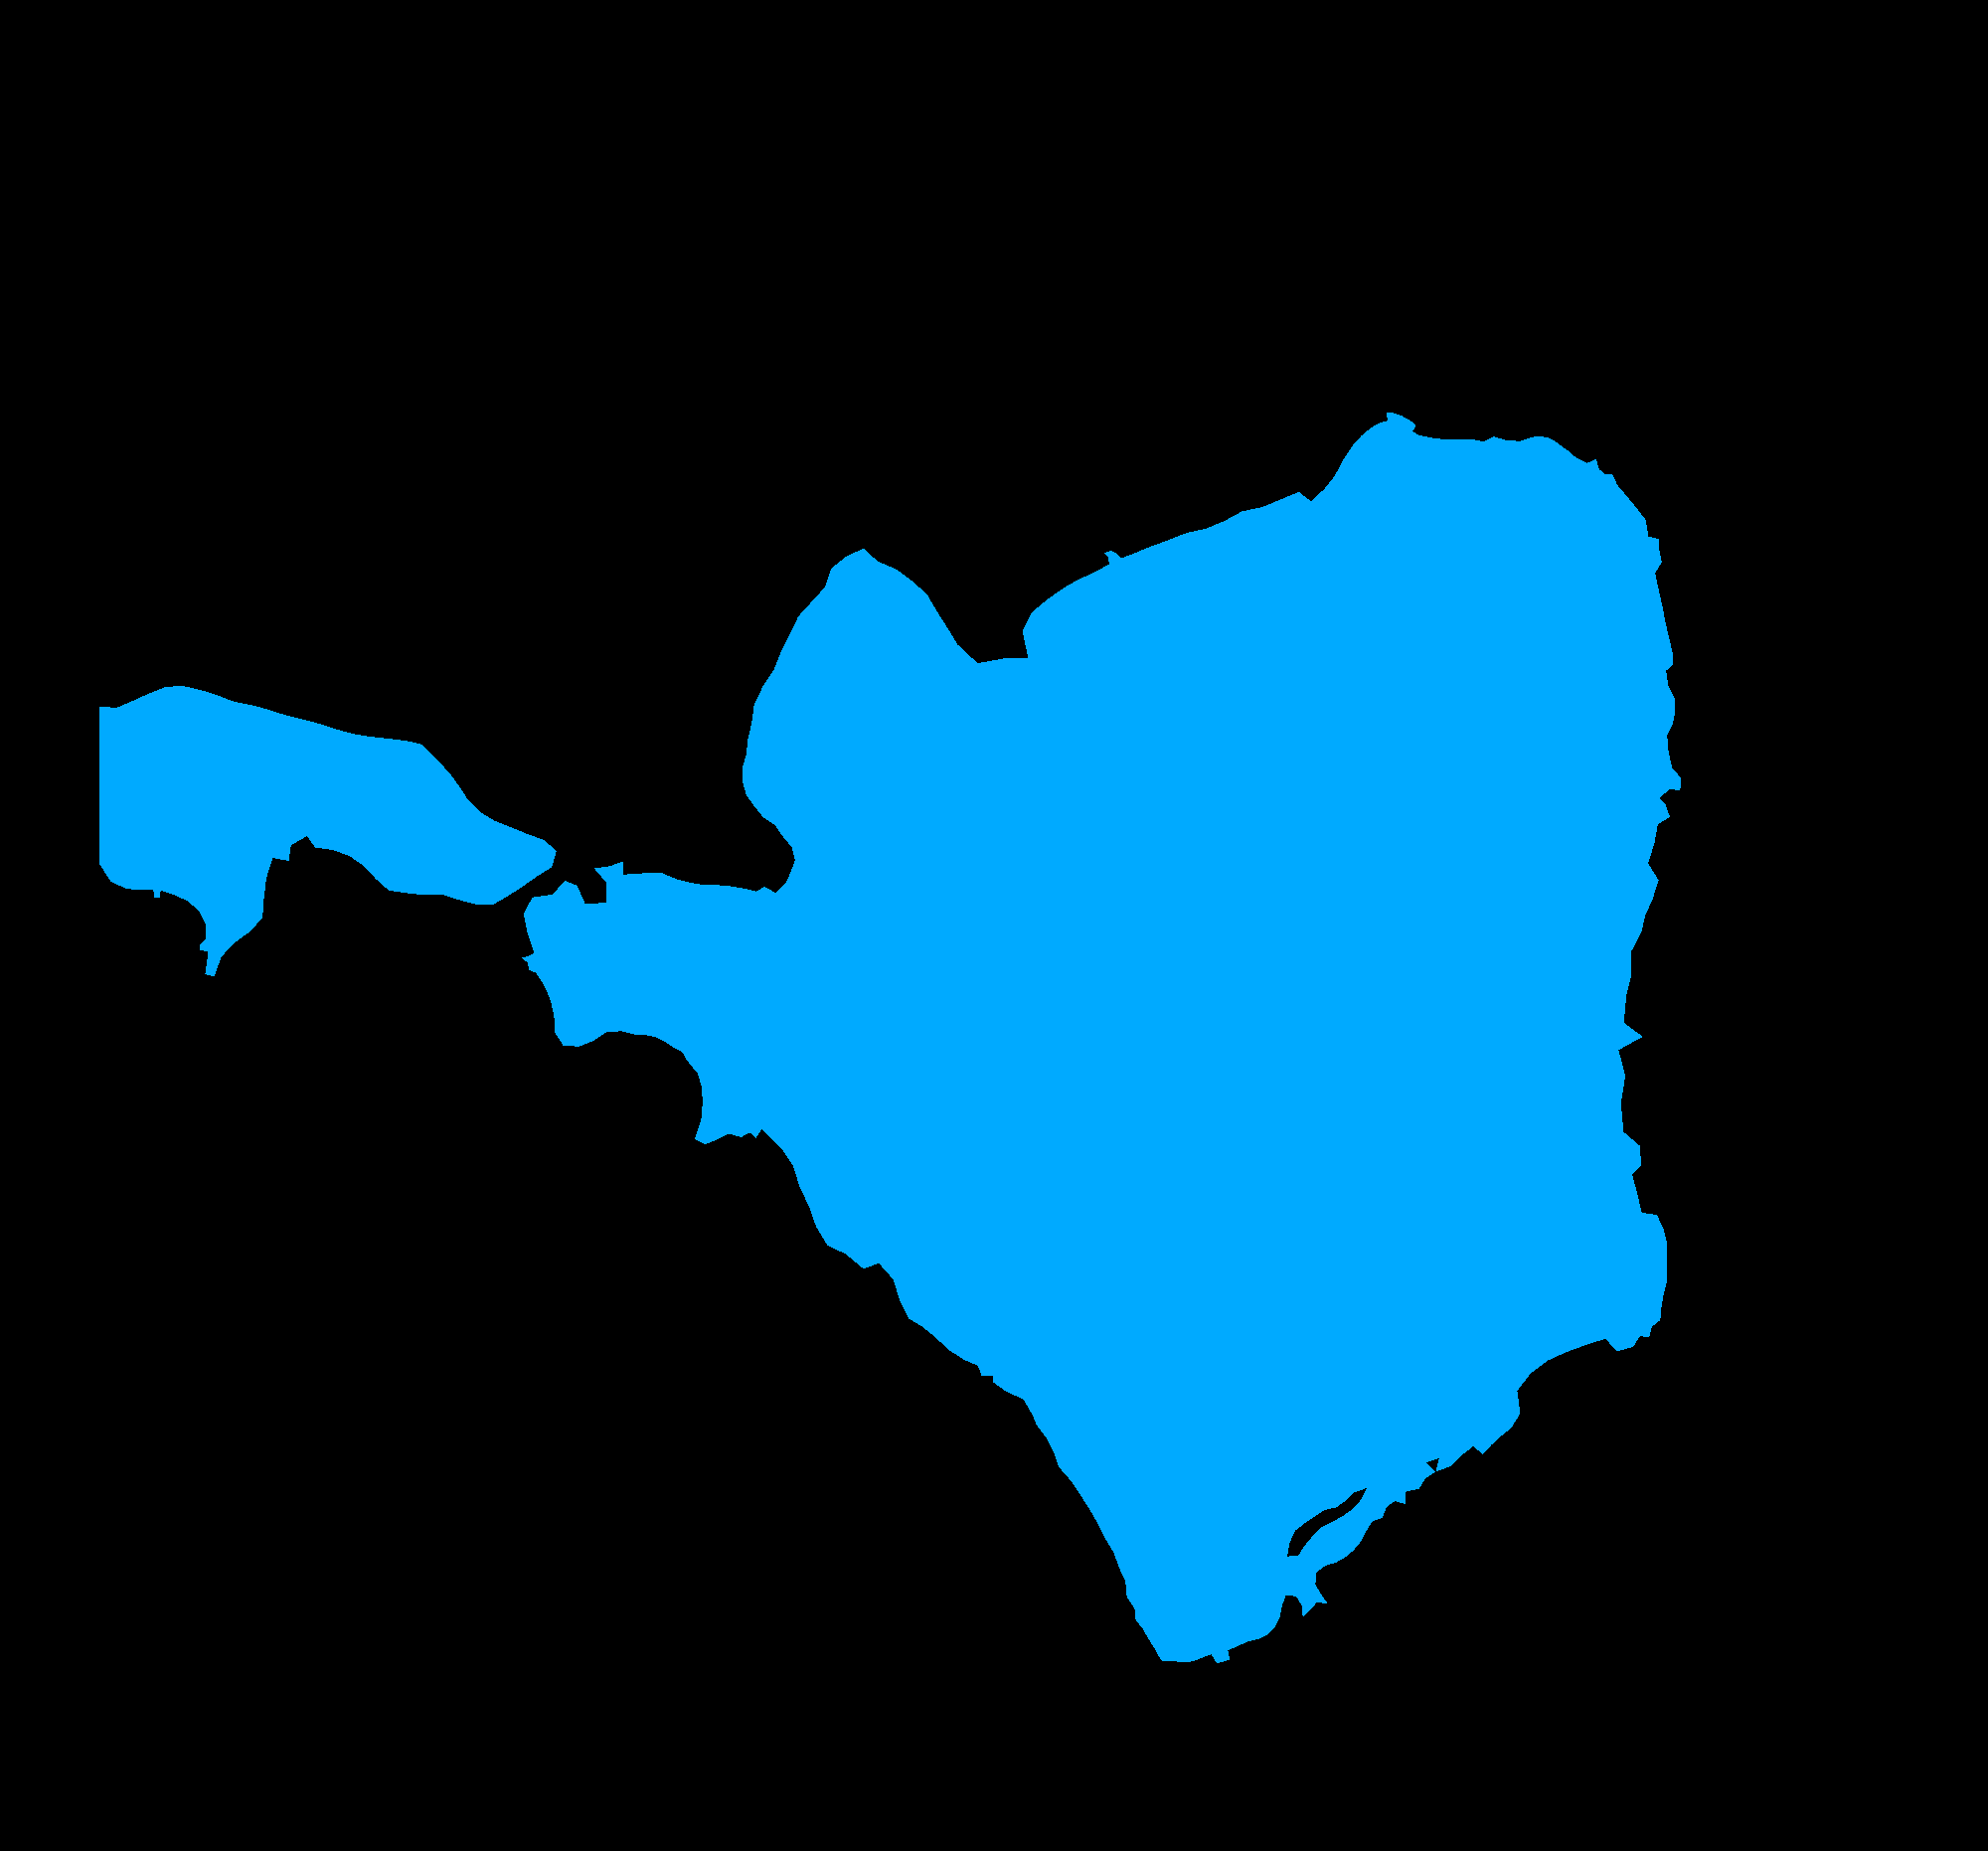
\includegraphics{franksTractZone600}
\caption{Resulted Franks Tract zone }
\label{figure:franksTractZone}
\end{center}
\end{figure} 	


With the pseudo-color plot is visible and selected as the figure \ref{figure:franksTractColorSelected}, go to VisIt main menu bar 
{\bf Controls}-$>${\bf Selections}. Click the {\bf New} button on the {\bf Selections} window to pop up {\bf Selection Name and Source}
window. Fill the name of the selection, and check the {\bf Plot} radio button for we are creating subset based on the current plot.
On the bottom of the {\bf Selection Name and Source} window, there are four options to project the selection point to other plot.
The first option {\bf Domain and cell numbers} are checked by default and this option is the correct choice if the plot or database in which selection is going to applied are using the same mesh. If this is not the case, {\bf locations} is a the better choice. When done with
the {\bf Selection Name and Source} window, don't forget to check the {\bf Automatically apply updated selections} on the botthom of the window
{\bf Selections}. The setup for the example Franks Tract is show in figure \ref{figure:franksTractSelections}. If any change made to
the file defining the selection user can update the subset by clicking the {\bf Update Selection} button on the right-bottom of the {\bf Selection}
windows.
 


\begin{figure}
\begin{center}
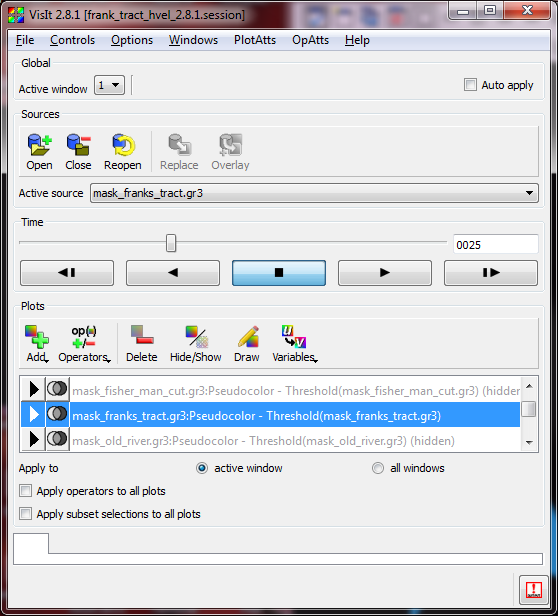
\includegraphics{franksTractColorSelected}
\caption{Plot selected }
\label{figure:franksTractColorSelected}
\end{center}
\end{figure} 	


\begin{figure}
\begin{center}
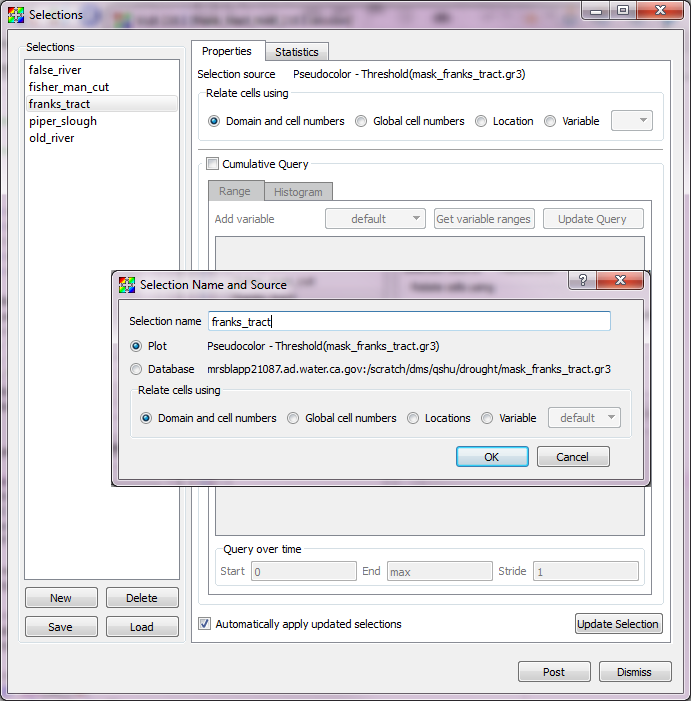
\includegraphics{franksTractSelections}
\caption{Selections setup }
\label{figure:franksTractSelections}
\end{center}
\end{figure} 	


Using the same operation other subsets can be defined, such as the subsets false\_river, fisher\_man\_cut, piper\_slough and old\_river shown
in the figure \ref{figure:franksTractSelections}.

Now, we would like to generate  vector and magnitude value plot of flow velocity over the all the zones. We want to apply dense vector over
the zone of Franks Tract to show its flow eddy pattern. On the other hand we want to the vector plot on the surrounding rivers are sparser without hiding flow magnitude color. This effect is achieved by doing a plot for each zone individually with different vector density setup.
The combination of all those subset plot will be looks like figure \ref{figure:franksTractCombinedVel}.

\begin{figure}
\begin{center}
\includegraphics{franksTractCombinedVel}
\caption{Resulting effect}
\label{figure:franksTractCombinedVel}
\end{center}
\end{figure} 	


First a vector plot of flow field over the whole domain as demonstrated in section \ref{subsection:viewstate}. 
With the plot selected, go to main menu {\bf Controls}-$>${\bf Subset}. To the bottom of the \emph{Subset} window,
choose the subset to be applied from the drop down list as shown in figure \ref{figure:subsetsApply}, then apply 
the selection.  Then configure the vector plot attributes as shown in by figure \ref{figure:denseVectorStyle} and
set the vector stride to 1.

\begin{figure}
\begin{center}
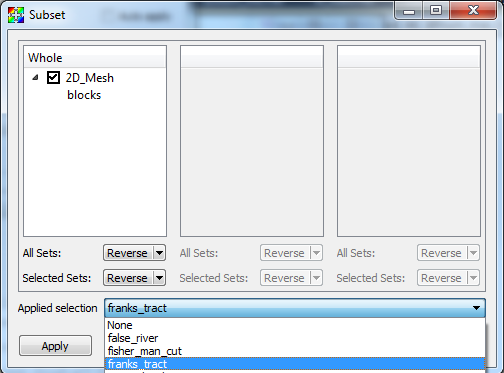
\includegraphics{subsetsApply}
\caption{Applying subset}
\label{figure:subsetsApply}
\end{center}
\end{figure} 

\begin{figure}
\begin{center}
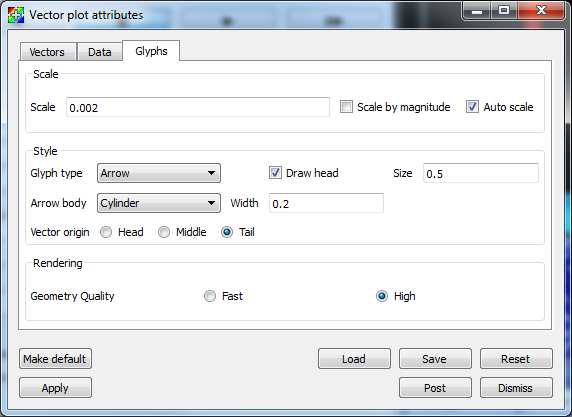
\includegraphics{denseVectorStyle}
\caption{Vector plot attribute with stride =1 }
\label{figure:denseVectorStyle}
\end{center}
\end{figure} 


Repeat those steps for other subsets but with different vector stride setup. Those jobs can be done quicker by first cloning
a vector plot then swapping the subsets applied to the plot.


Another small application of subsetting is to plot boundary of a 2D mesh. Suppose a data file is open already, go to plots menu {\bf Add}-$>${\bf Subset} and choose {\bf 2D\_Mesh} as shown in figure 
\ref{figure:subsetBounaryMenu}, then click {\bf Draw} button on the plots menu.After 2D mesh is plot, go to main menu {\bf PlotAtts}-$>${\bf Subset}. On the middle of the \emph{Subset plot attributes} window,
check \emph{Wireframe} on the \emph{Options} panel as shown by the red box in figure 
\ref{figure:subsetBoundaryAtts}, then apply the option.  The boundary is as shown in by figure 
\ref{figure:subsetBoundaryPlot}.

\begin{figure}
\begin{center}
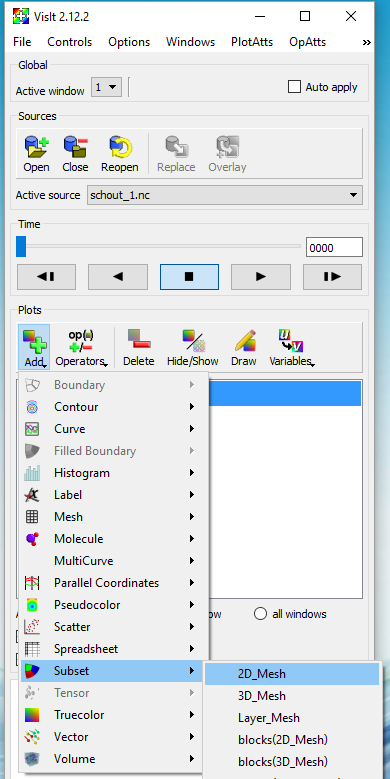
\includegraphics{subsetBoundaryMenu}
\caption{Subset boundary plot menu}
\label{figure:subsetBounaryMenu}
\end{center}
\end{figure} 

\begin{figure}
\begin{center}
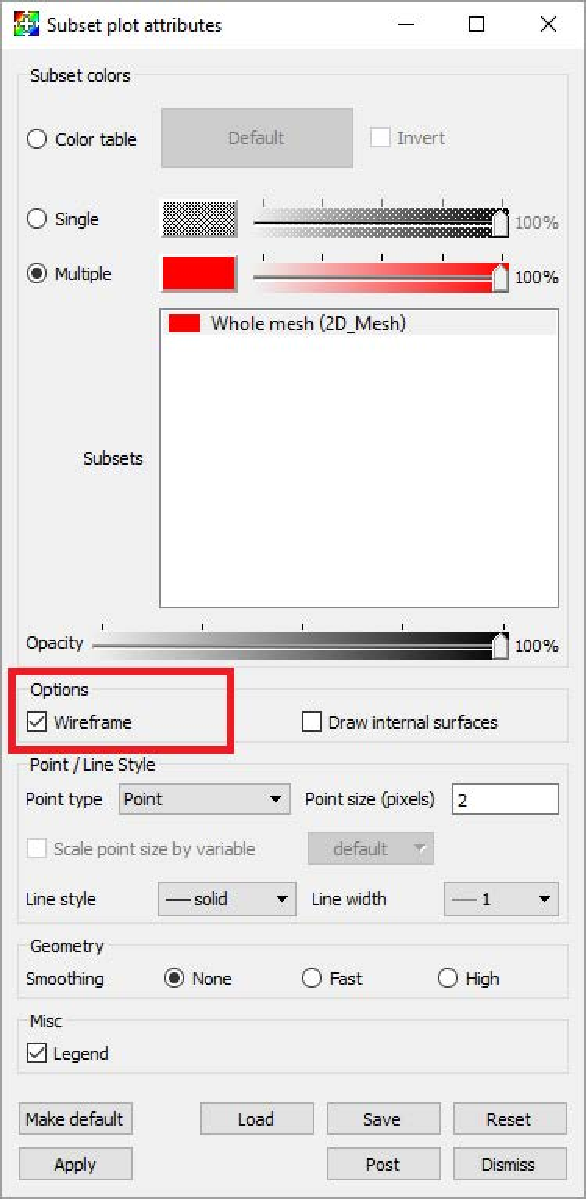
\includegraphics{subsetBoundaryAtts}
\caption{Subset boundary plot attribute }
\label{figure:subsetBoundaryAtts}
\end{center}
\end{figure} 

\begin{figure}
\begin{center}
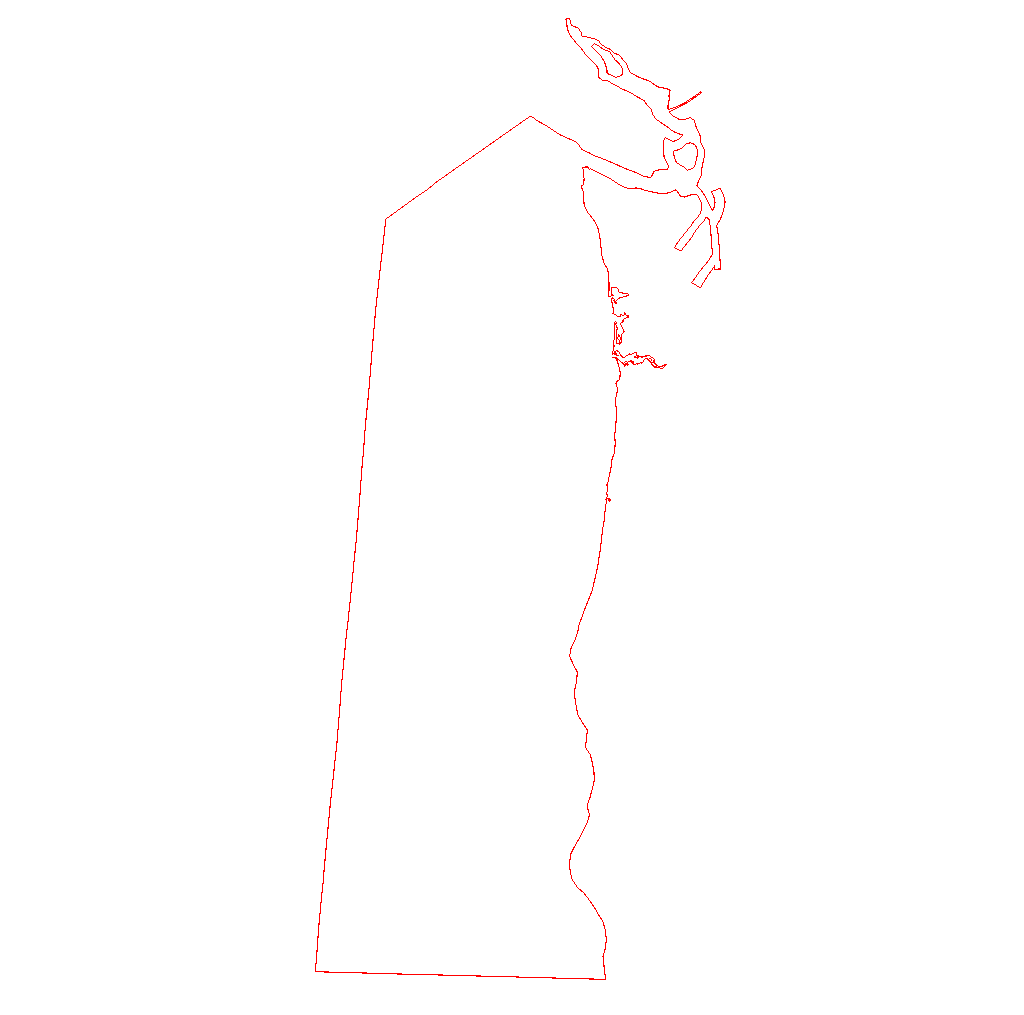
\includegraphics{subsetBoundaryPlot300dpi}
\caption{Boundary plot}
\label{figure:subsetBoundaryPlot}
\end{center}
\end{figure} 



\section{Time Iteration Functions}

There are a number of time iteration function available to extract some interesting values from a dataset, such as
daily maximum/minimal values on each mesh node. The figure \ref{figure:timeFunctions} shows menu of those time functions.

\begin{figure}
\begin{center}
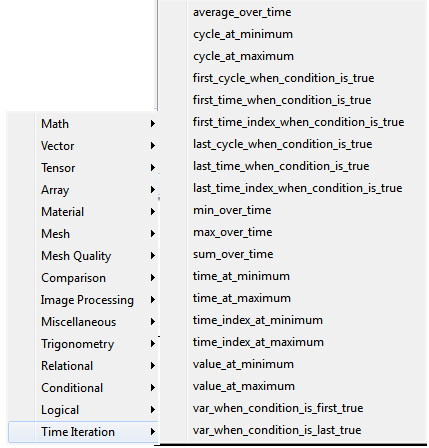
\includegraphics{timeFunctions}
\caption{Time iteration menu }
\label{figure:timeFunctions}
\end{center}
\end{figure} 

Time functions can be accessed from VisIt expression building window. Go to main menu {\bf Controls}-$>$ {\bf Expressions}.
The {\bf Expression} window will be looks like  \ref{figure:timeExpression}. The expression defines the maximal surface value
on each node of the mesh in the time span from step 0 to  step 71 with time stride of 1. The result of the expression can be
export as a database storing data and graphic rendering information as well, for instance VTK file. The exported database can
be reopened using VisIt for further operation, such like comparing result of different numerical model setup. 

\begin{figure}
\begin{center}
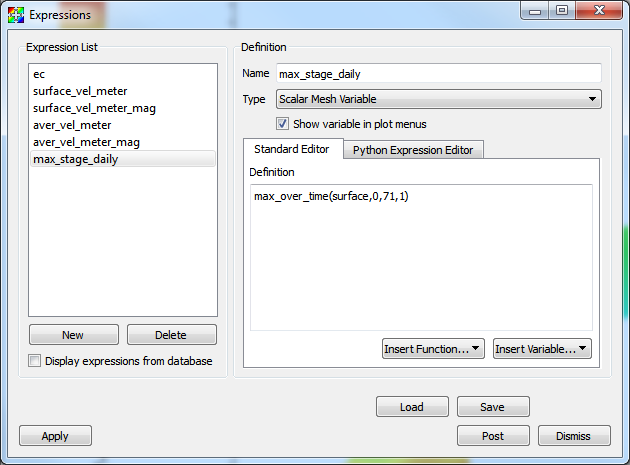
\includegraphics{timeExpression}
\caption{Time iteration expression }
\label{figure:timeExpression}
\end{center}
\end{figure} 







\chapter{Example: Salinity Plot and Animation}
	
This section builds on the salinity example in section \ref{subsection:viewstate},
demonstrating some steps you can go through to make your output 
simpler and more professional. The final product is a visualization of salinity
intrusion in a region near 2 ppt (x2) in the Sacramento-San Joaquin Delta. 

\section{File Grouping}
	
For the example, we will use the same grouping strategy described in \ref{sec:time} 
using a \emph{.visit} file to indicate the sequence of time in the  animation. 
Below is a example of a file \emph{.visit} file for a group of salt output files. 
We named it after the start and end day, but the .visit extension is the only required 
part of the name:
		
\begin{verbatim}
====== File salt_200_216.visit =======
		   200_salt.63
       201_salt.63
       202_salt.63
			  ... 
       215_salt.63
       216_salt.63
====== End of file ====
\end{verbatim}
		
	
After creating your \emph{.visit} file, open it in SCHISM format using {\bf Open \textrightarrow File} 
just as you would for a binary files. Visit will automatically check all the output files, 
counting the total number of time steps available. After counting is done, you will 
see a time slide control available on the Visit main interface as shown in Figure \ref{figure:timeVCR}.
			
			  \begin{figure}
        \begin{center}
        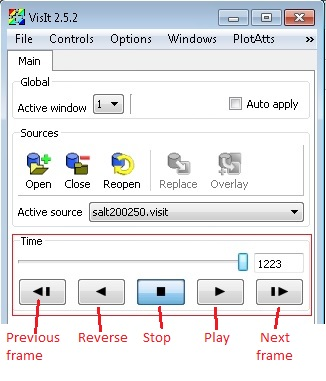
\includegraphics{timeVCR}
        \caption{Time slider}
        \label{figure:timeVCR}
        \end{center}
        \end{figure} 
				
Similar to a DVD player in appearance, the button under the time slider can be used to navigated among the time steps of the output files or play the animation continuously.  You can also drag the time slider to the 
desired time steps or input the time steps on the box next to the time slider. We have found it
best important to let VisIt finish what it was trying to do and to stop it before operations such as zooming.
Also, be mindful of endlessly looping animations as this draws down memory -- this is something we think
may be fixed in future versions and we have reported it to LLNL.
			
			
\section{Refining the Appearance}
			
This section builds on the salinity example in section \ref{subsection:viewstate},
demonstrating some steps you can go through to make your output 
simpler and more professional. The final product is a visualization of salinity
intrusion in a region near 2 ppt (x2) in the Sacramento-San Joaquin Delta. 
			
\subsection{Masking Dry Elements}
The starting point is section \ref{subsection:viewstate}, which shows how to create a basic 
{\bf Pseudocolor} plot of bottom salinity (\emph{salt\_bottom}) from a SCHISM output database.
	
For most simulations, some subset of elements will inevitably be dry and be filled with large 
negative salinity values which are the default fill value for dry elements. You can mask out 
dry cells using {\bf VisIt Threshold} selection operator. Details of this operation are given in section \ref{sec:thresholdOperator}. The lower bound chosen for this plot is 0.01, and there is upper bound restriction.
			
Some of the Pseudocolor plot attributes are shown in the Figure \ref{figure:saltColorAttr}. Our 
visualization was originally intended to focus attention on on the 2ppt isohaline. This value,
referred to locally as X2, is of regulatory and ecological interest. So we used a divergent three color scheme
with the middle value falling at 2 psu which is equivalent. That value isn't quite appropriate for the scale here, so we
are centering the legend at half that value (1 psu).
	
			  \begin{figure}
        \begin{center}
        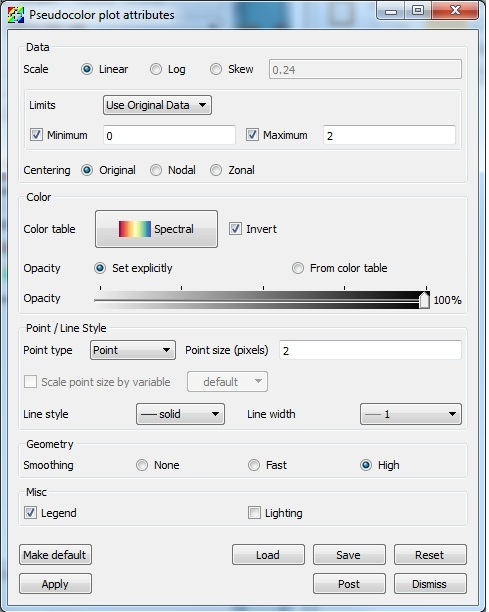
\includegraphics {saltColorAttr}
        \caption{Plot attributes of for a plot of bottom salinity near X2.}
        \label{figure:saltColorAttr}
        \end{center}
        \end{figure} 
				
				
\subsection{Plot Annotations}
			 
We usually override most of default annotation options, getting rid of some that are confusing (like "`pseudocolor"' and 
adding context labels. Select the {\bf Controls} menu on the main toolbar and click on the menu item {\bf Annotation} to show 
the Annotation option windows. Uncheck the option {\bf Database}, {\bf Time} and {\bf User information} on the {\bf General} property sheet, as shown in Figure \ref{figure:annotationGeneral}. In addition, for this example we don't to show axis in the plot; hence, the option {\bf Show axes} on the {\bf 2D}  property sheet is also unchecked. Leave the dialog open.
			
			  \begin{figure}
        \begin{center}
        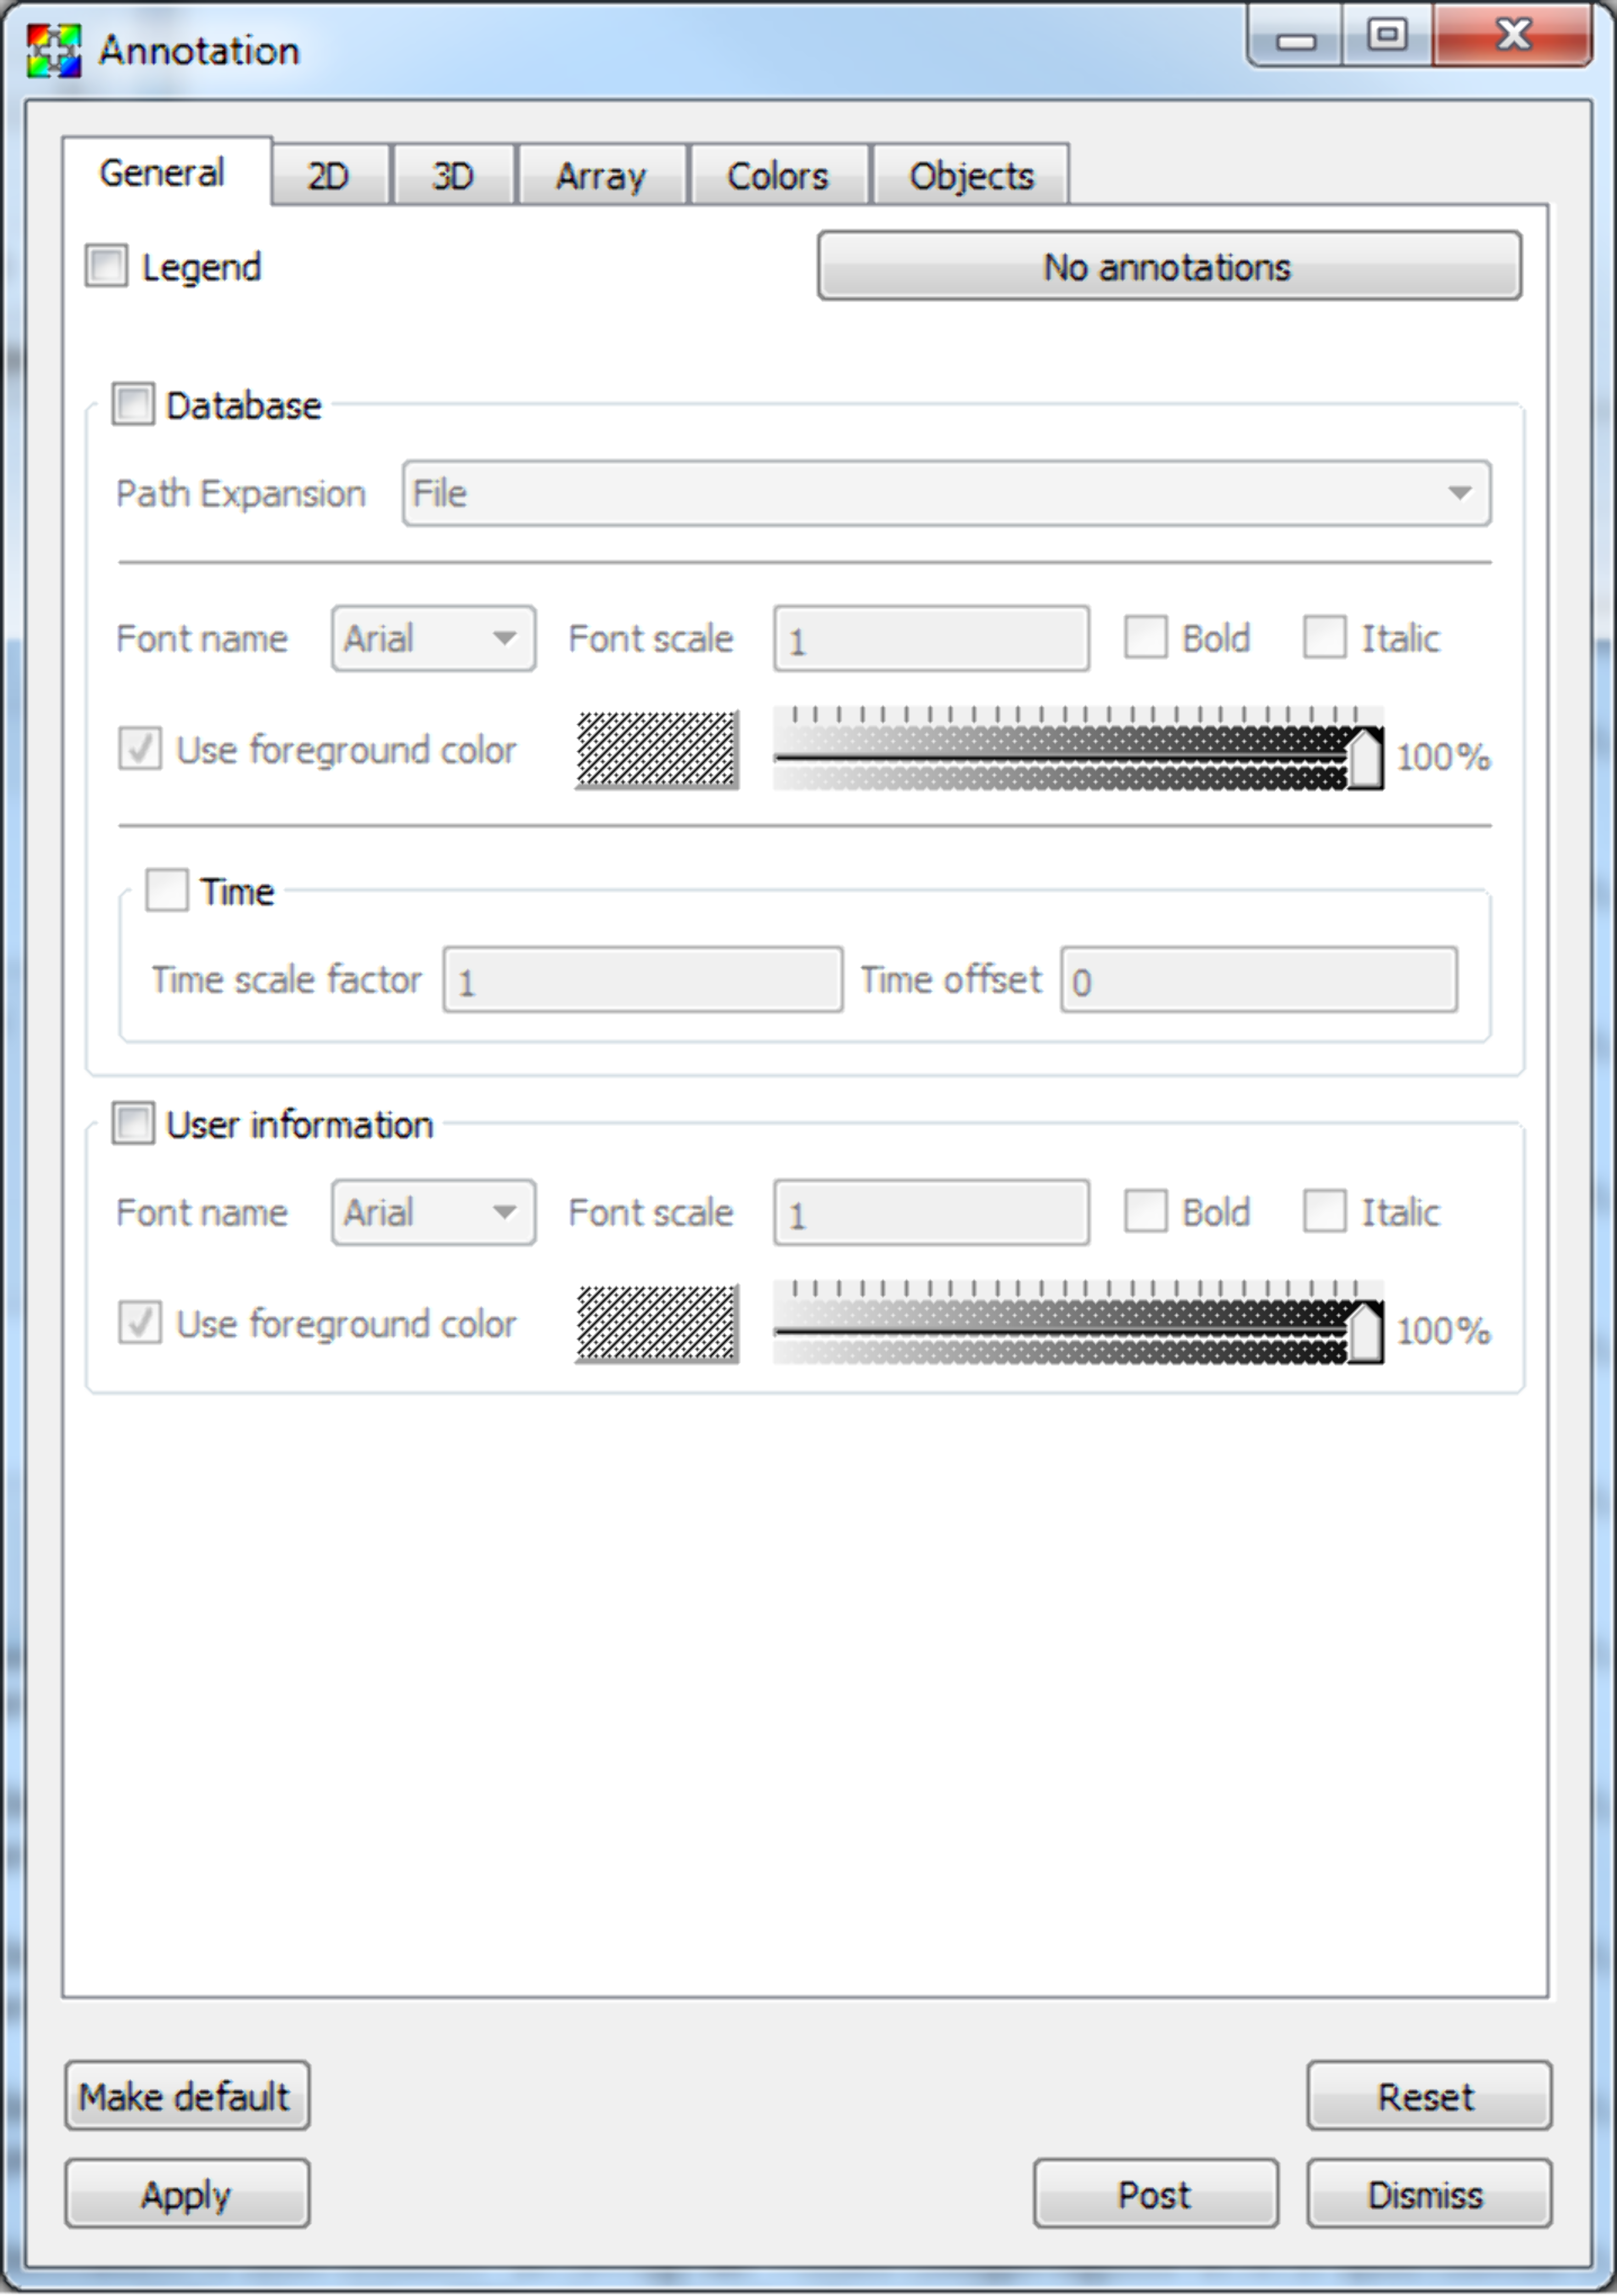
\includegraphics{annotationGeneral}
        \caption{Annotation options}
        \label{figure:annotationGeneral}
        \end{center}
        \end{figure} 
			
Next, we are going to display a customized horizontal legend for the salinity plot. 
In the Annotation attribute window, click on  the {\bf Objects} tab. There should be a item 
called {\bf Legend:Pseudocolor\-Threshold(salt\_bottom)} in the list of {\bf Annotation objects}. 
Click on this item and the lower part of attribute sheet will display the attributes related to this item. 
There are three attribute sheets with the names {\bf Position},{\bf Tick Marks} and {\bf Appearance}.
				
On the {\bf Position} attribute sheet, uncheck the option {\bf Let VisIt managed legend position} to enable
the position adjustment options shown in Figure \ref{figure:legendAttrPos}. You can input the desired
location in screen coordinates and select an orientation. You may have to employ some trial and error; 
the value shown on the Figure \ref{figure:legendAttrPos} are the ones used for this example. 

	      \begin{figure}
        \begin{center}
        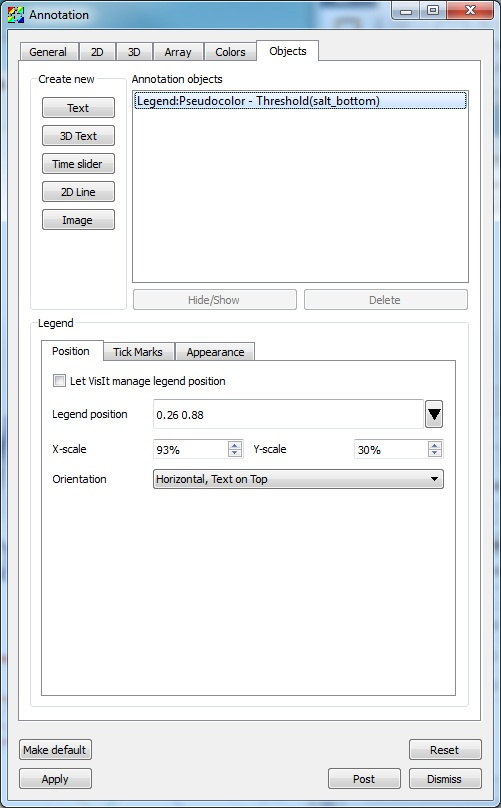
\includegraphics{legendAttrPos}
        \caption{Legend location}
        \label{figure:legendAttrPos}
        \end{center}
        \end{figure}
				
				\begin{figure}
        \begin{center}
        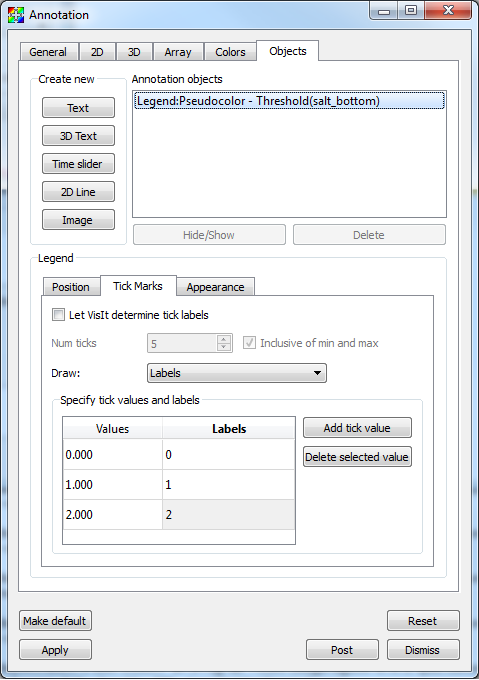
\includegraphics{legendAttrTicks}
        \caption{Legend ticks}
        \label{figure:legendAttrTicks}
        \end{center}
        \end{figure} 
				
In this example, we only want to display labels at 0, 1 and 2 psu and we want to draw our labels without
any figures after the decimal point. 
To get this effect, click on the {\bf Tick Marks} tab to activate Tick attribute sheet and uncheck the option 
{\bf Let VisIt determine tick labels}. Then select {\bf Labels} from the {\bf Draw} Drop-down list. 
Delete all the default ticks values from the table in the lower part of the sheet.  Then click on 
the button {\bf Add tick value} to add new tick values and corresponding labels on the table.  
Figure \ref{figure:legendAttrTicks} shows the ticks marks setup for this example.
				
				\begin{figure}
        \begin{center}
        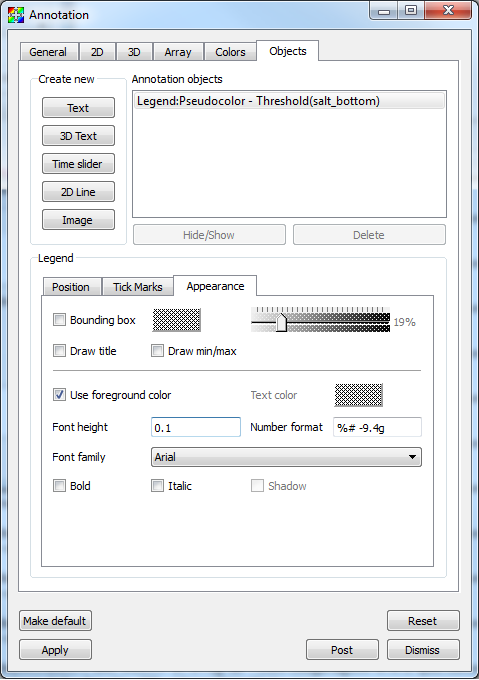
\includegraphics{legendAttrAppear}
        \caption{Legend appearance}
        \label{figure:legendAttrAppear}
        \end{center}
        \end{figure} 
				  
You can choose the legend font family, size and some appearance on the attribute sheet {\bf Appearance} as shown in
Figure \ref{figure:legendAttrAppear}. For this example, we hide the default legend title. We will replace it with our
own legend tile by creating a new text annotation on the annotation 
object attribute sheet as shown in Figure \ref{figure:textObject}. 

You may need to adjust the text object location,
size and color to accommodate existing legend objects. 
Figure \ref{figure:textObject} shows the text attributes used  
for the example. In addition two labels indicate water saltiness are placed under
to create the legend. The final legend can be seen in the Figure \ref{figure:legendProduct}.
				
				\begin{figure}
        \begin{center}
        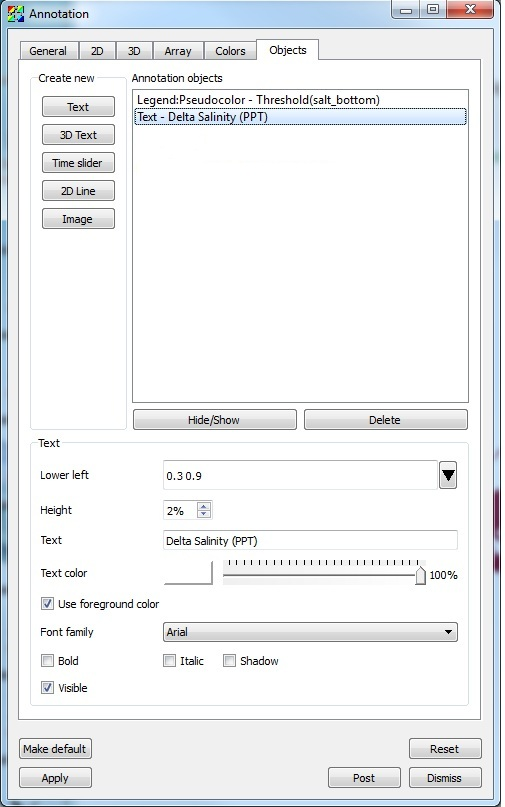
\includegraphics{textObject}
        \caption{Adding text object}
        \label{figure:textObject}
        \end{center}
        \end{figure} 
				
				
				\begin{figure}
        \begin{center}
        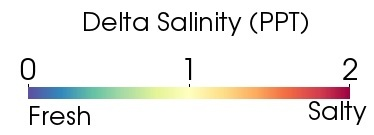
\includegraphics{legendProduct}
        \caption{Legend product}
        \label{figure:legendProduct}
        \end{center}
        \end{figure} 
			
			
			\subsection{Plot Background}
			
In this step, we use a background image to label some interest geographical points. In principle this can be done with
annotation but the result is usually difficult to manage under panning and zooming and doesn't look as good as the technique
described below using georeferenced images.
			
You can create a georeferenced background image containing only text labels using third party tools, such as ArcGIS or GDAL. That subject is beyond the scope of this tutorial, but an easy search on the web. The image file  should be geo-referenced. In this example, we use a png image file accompanied by a pgw file, which contains the georeferencing information. 
VisIt supports the import of geo-referenced images through the GDAL plugin. 
Figure \ref{figure:openGeoPng} shows how to open a georeferenced png file as GDAL format file. 
						
\begin{figure}
\begin{center}
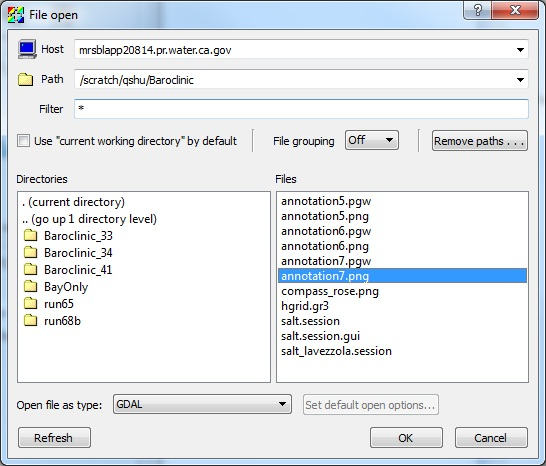
\includegraphics{openGeoPng}
\caption{Open background image}
\label{figure:openGeoPng}
\end{center}
\end{figure} 
				
After the background image file is opened successfully, the active source drop-down list on the main  VisIt window should switch to the image file automatically. 
If not, select the image file just opened from the drop-down list. To display all 
the labels in the background image, you will add a {\bf Truecolor} plot. To add a {\bf Truecolor} plot of the image file,
click on the {\bf Add} button on the {\bf Plots} panel of the main window , then move to {\bf Truecolor} menu and 
{\bf color} submenu item. VisIt should then render the background image on the active display window.
				
For the example background image, a {\bf Threshold} operator can be applied to filter out some undesired original image pixels and make image neater.  The setup of of the {\bf Threshold} is shown as Figure \ref{figure:backgroundThreshold}.
				
				\begin{figure}
        \begin{center}
        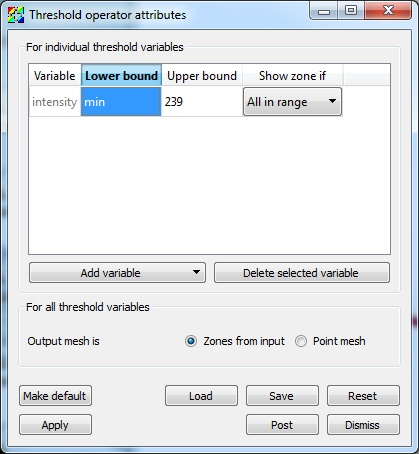
\includegraphics[scale=0.75]{backgroundThreshold}
        \caption{Background image setup}
        \label{figure:backgroundThreshold}
        \end{center}
        \end{figure}
				
The resulting plot should look something like Figure \ref{figure:saltWithBackground}. Users may need to adjust display zooming to fit their own purposes.
				
				\begin{figure}
        \begin{center}
        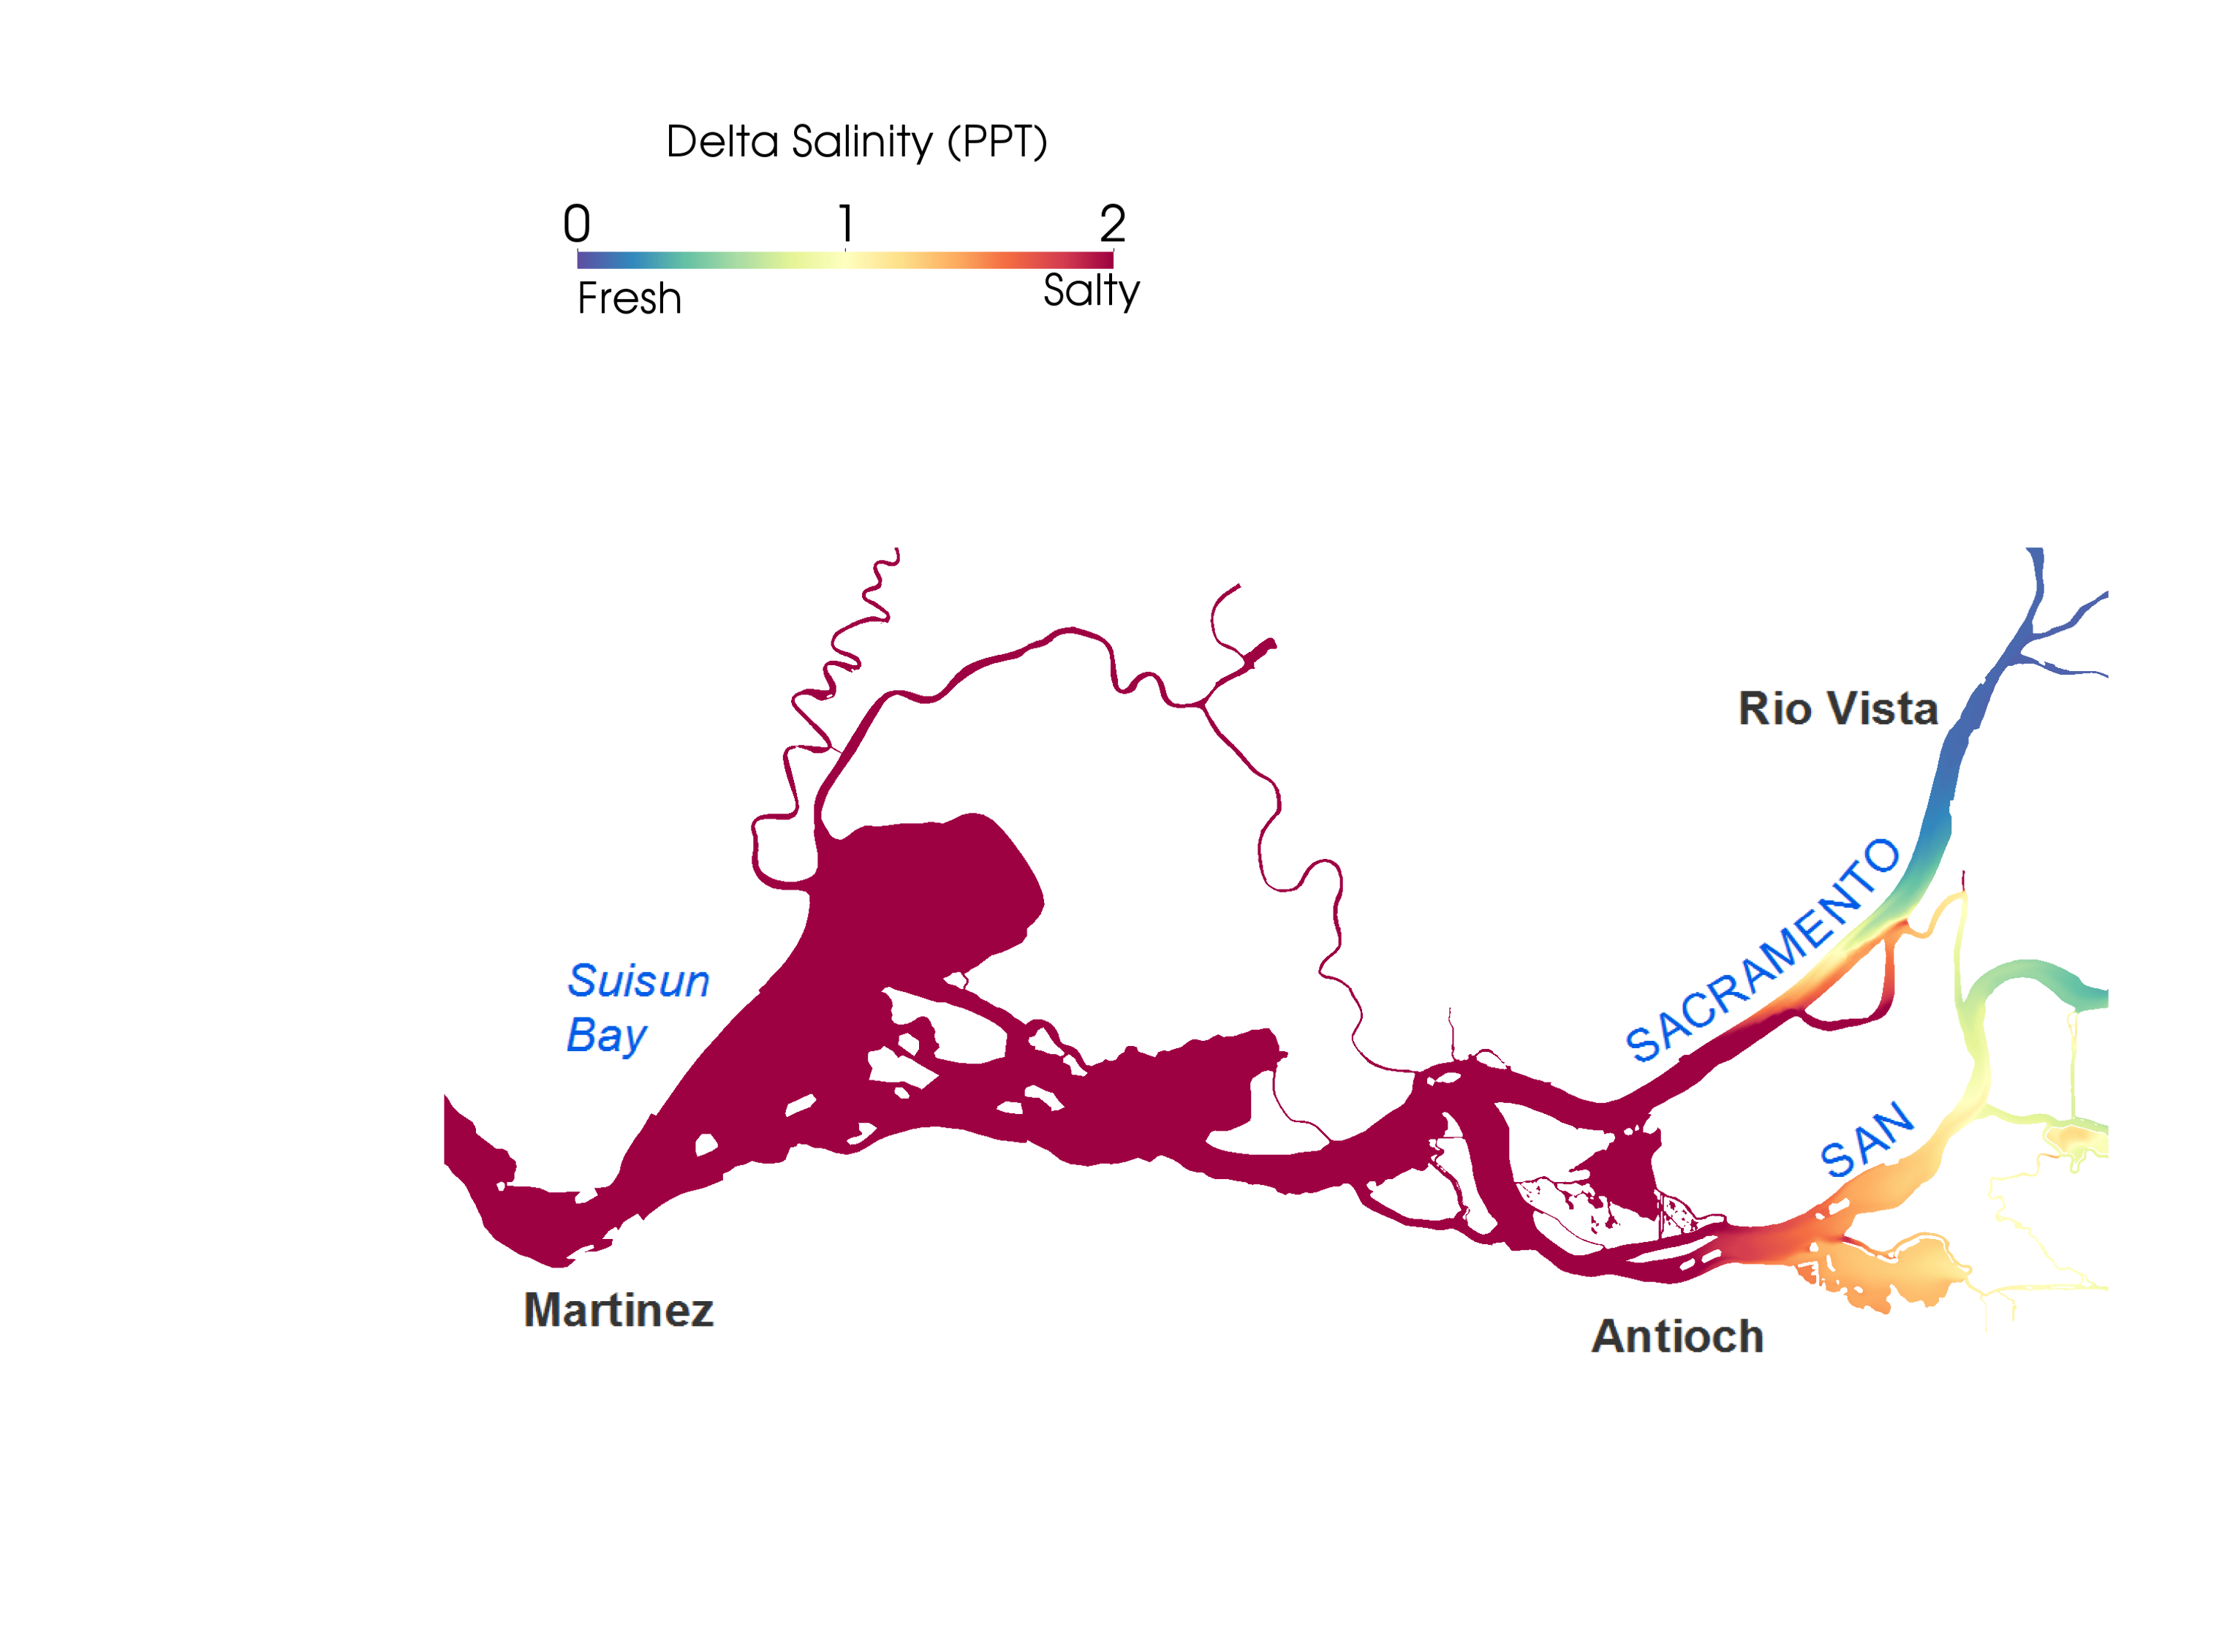
\includegraphics[scale=0.15]{saltWithBackground}
        \caption{Plot with background labels}
        \label{figure:saltWithBackground}
        \end{center}
        \end{figure}
				
				\section{Creating an Animation }
				
				Although VisIt can create animation files directly from output databases files, you will get better quality
				if you use VisIt to generate high resolution image files from all the time steps and then create the animation movie 
				a specialty tool like the ImageMagick ffmpeg (for mp4) or Microsoft movie maker. To create movie image files,
				select {\bf File} and {\bf Save movie} to show {\bf Save movie wizard}. In this example, we will
				create a simple movie, which is the default option as indicated in Figure \ref{figure:movieWizardSimple}. 
				
				\begin{figure}
        \begin{center}
        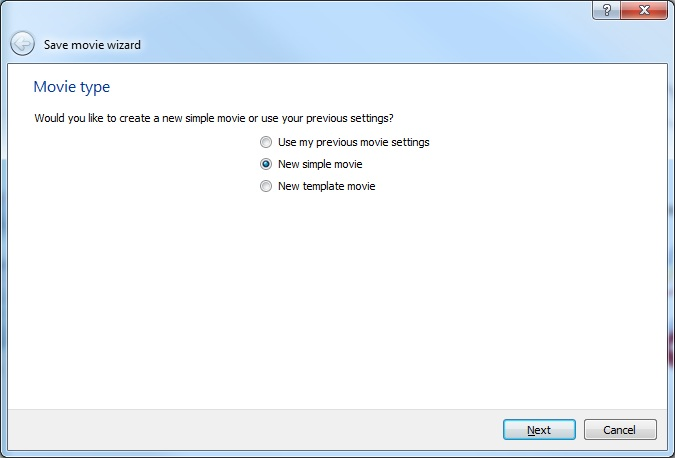
\includegraphics[scale=0.75]{movieWizardSimple}
        \caption{Simple movie}
        \label{figure:movieWizardSimple}
        \end{center}
        \end{figure}
				
				After choosing the simple movie template, choose the movie format as shown in Figure \ref{figure:movieFormat}.
				
				\begin{figure}
        \begin{center}
        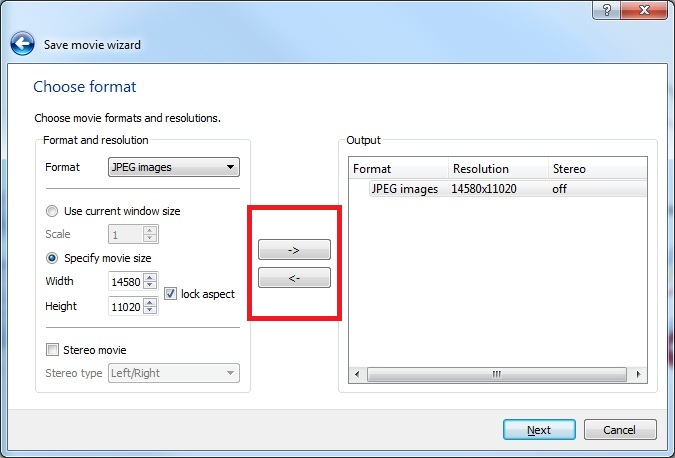
\includegraphics[scale=0.75]{movieFormat}
        \caption{Movie format}
        \label{figure:movieFormat}
        \end{center}
        \end{figure}
		    
On the movie format window, choose {\bf JPEG images} from the {\bf Format} dropdown list 
since we are creating animation image files. You will need to set the movie image 
resolution by specifying movie width and height. After choosing the image format and
size, user must click on the {\bf "-$>$"} button to save the configuration to the {\bf Output} table. If user want delete a 
configuration, just highlight the configuration entry in the {\bf Output} table and click on the {\bf "$<$-"} button. If there are more than one configuration entries saved in the {\bf Output} table, the one highlighted will be used. To avoid confusion it is good practice to keep only one entry in the table.
				
After finishing the movie format configuration, choose the length of the animation. VisIt will automatically fill the starting and ending frames, which are the beginning and ending of the databases respectively. 
User may accept this default length, or change to fit
his/her purpose.  This window is shown in Figure \ref{figure:movieLength}.
				
				\begin{figure}
        \begin{center}
        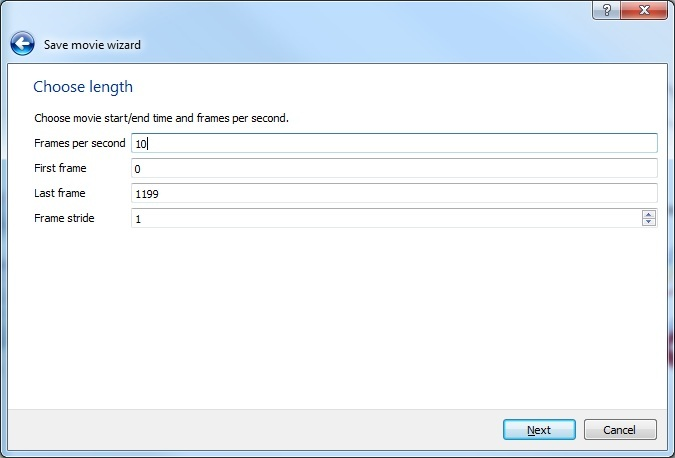
\includegraphics[scale=0.75]{movieLength}
        \caption{Movie length}
        \label{figure:movieLength}
        \end{center}
        \end{figure}
				
				Next, user may need to specify a base filename for the output image files as shown in Figure \ref {figure:movieName}.
				\begin{figure}
        \begin{center}
        \includegraphics[scale=0.75]{movieName}
        \caption{Movie name}
        \label{figure:movieName}
        \end{center}
        \end{figure}
				
Typically you can accept the defaults for the rest of the configuration. 
After these setup steps, VisIt will start creating image files 
and saving them to the location specified by the user.
				
\subsection{Creating the animation}
When all the image files have been created, you can create animation using 
a tool such as ffmpeg from ImageMagick (a command line operation) or 
Microsoft Movie Maker. The choice between these two tools will depend on how
good you want your movie to be and where you want to show it and whether you 
want a graphical interface. Movie Maker creates {\em *.mov} animations 
of acceptable quality that are highly portable between
Windows computers and has a simple graphical interface. The online documentation 
and tutorials for Movie Maker are plentiful so we won't repeat that here.

The {\em mp4} format is portable over a larger variety of platforms and produces
somewhat better images with more economical file sizes. For this format, the 
command line tool ffmpeg from ImageMagick is very helpful. Actually it can produce
.mov files as well as .mp4.

\subsubsection{Basic ffmpeg Recipes for Animations}
The following are commands for generating mp4 or mov files in ffmpeg from still images (png). Keeping the ordering of the options is important. As a general rule, options are applied to the next specified file. 


\paragraph{mp4}
For MP4 animations, the following command (all on one line) works well, producing high quality graphics:
\begin{verbatim}
$ffmpeg -i afile_%04d.png -r 10 -b 4000k -mbd rd -flags +mv4+aic
 -trellis 2 -cmp 2 -subcmp 2 -g 300  output.mp4 
\end{verbatim}
where:
\-i names the input. The base name {\em afile\_} is arbitrary and \%04 indicates successive digits \\ 
\-r is the frame rate. The lower it is, the faster the movie goes but it will have a tendency to jump around as well. You cannot fully control speed and quality with just the frame rate – this depends on the time resolution of your images as well. If you specify a very high frame rate, it will duplicate frames and take just as long. If you specify a low rate it will drop frames. \\
\-b 4000k sets the bit rate, which will affect the quality of the output \\
and all the other flags are optimizations for mp4 quality and should probably always be used. 

\paragraph{mov}
To create a wmv format animation from files named using the pattern 'img0000.png', use:
\begin{verbatim} 
ffmpeg -r 10 -i img%04d.png -b:v 392k -r 10 movie.wmv
\end{verbatim}
With the variable bitrate of 392kbps in option '-b:v', which decides the compression ratio, the quality will probably be good enough without seriously noticeable artifacts. The frame rate in first '-r' option decides how fast images flip to the next one. The option '-i' provides input files. The codec in this case will be inferred from the output file extension. 


								
\subsection {Editing Animation Images and Calendar Timestamps}

There are often times when you will want to add custom images or calendar timestamps
to your images. A prime example of this is the calendar time stamp. Both VisIt 
and SCHISM operate on elapsed seconds, which is meaningless to most audiences.
Imprinting a datetime can help viewers relate the visualization to 
calendar time. 

Similarly, you may want to add a customized icon, for instance a compass rose or branding.
VisIt does provide for static i

A python code is list in appendix \ref{append:stampImages}. User may need to make change to fit his/her own use cases.
				
				
\section{VisIt Session Files}
				
VisIt enables users to save data source, formatting, annotations and display 
choices into a session file that can be reloaded and resumed later. 
You can also restore a session and file and apply it to new data.
To save a session, choose {\bf File \textrightarrow Save session} menu item. 
				
To reload a existing session file, choose {\bf File \textrightarrow \bf Restore session} the
menu item, then navigate to the location *.session file you want to restore.
VisIt will reload the data sources and recover all the plot and styles saved
in the session file. You may need to re-authenticate if an ssh connection is
used to connect to a remote server. 
								
After loading a session file, you may choose to switch to a different data source or 
database, say another \emph{.visit} file.
To do this, open the new data source file then 
replace the active source with the new data file. 
					
				
Occasionally, VisIt may fail to load a session file and complain about a metadata error. 
If this happens, you should repeat the steps and VisIt will finished the job after a couple seconds.


\chapter{Discussion}

\section{Dry Cell Handling}

 In the legacy binary output file, elevation of the levels above bed on a dry cell are set to 0.0. VisIt plugin uses the
value to build vertical mesh directly. For the NC4 format output, elevation of the levels above bed on a dry cell are set to nonphysical filling value. VisIt can't handle those nonphysical value gracefully, instead a synthetic surface elevation ,0.0, is assumed on the dry cells for visualizing purpose only. The SCHSIM output plugin uses this synthetic surface to compute synthetic elevations for all the levels above the bed on a dry cell. It uses the same formula implemented in the SCHSIM code to convert S coordinates into Z elevations.

\section{S coordinate and Localized Sigma Coordinate}

 The SCHISM output plugin doesn't discriminate the output from those two vertical coordinate systems. VisIt can generate degenerated 3D prism
resulting by the different number of sigma levels of neighboring element.

\section{Static and Dynamic Vertical Mesh}

 The SCHISM output plugin can handle change of a 3D mesh in vertical direction. This change is limited to number of vertical levels and elevations. Such a scenario only apply to NC4 output file, binary output file is treated as static mesh always. The plugin looks for a global attribute flag in a NC4 output file, which is 0 for static and 1 for dynamic vertical mesh. For static case, plugin build the 3D mesh for one time and it reads in new elevations on node and update the 3D mesh elevations for new time steps. For dynamic case, the plugin checks for possible change of vertical mesh by comparing number of valid levels on a node to the one of previous step. If there is a change, it rebuilds the 3D mesh. If no change, it updates elevations only.

\section{State on Dry Cells}

  The plugin doesn't honor the state value on dry cells loaded from NC4 output file, it always display state of dry cells as NULL. For the binary output case, it will plot the state value on dry cells, which is usually set to -99.0 (temp, salt), 0.0 (nodal horizontal/vertical vel, zcor, other).
	
\section{Unstructured Meshes Generation}
	
	The SCHISM output plugin loads horizontal mesh element nodes, nodes vertical coordinates on valid levels and element/node bottom level index from output files to build the 2D/3D mesh. 

  The 2D mesh is a collection of triangle or quadrilateral shapes, generated by SCHSIM mesh element and nodes X,Y data directly. 
	
	The 3D mesh consists of four type of element VTK\_TERA, VTK\_PYRAMID, VTK\_WEDGE and VTK\_HEXAHEDRON shown in Figure \ref{figure:3dElements}.
				
				\begin{figure}
        \begin{center}
        \includegraphics[scale=0.75]{Element3D}
        \caption{Unstructured Cells}
        \label{figure:3dElements}
        \end{center}
        \end{figure}
				
	The plugin generates 3D mesh elements in layer by layer manner from the model bed to the surface. For each element on a layer, the plugin find out the number of nodes on the 3D element bottom based on the , and choose a correct type of 3D element to be created. Here is a summary of decision for triangle and
quadrilateral mesh element:
	
\emph{Quadrilateral element}

\begin{enumerate}
\item  4 valid nodes on bottom, use VTK\_HEXAEDRON 
\item  3 valid nodes on bottom, use VTK\_HEXAEDRON
\item  2 valid nodes on bottom, use VTK\_EDGE
\item  1 valid nodes on bottom, use VTK\_PYRAMID
\end{enumerate}


\emph{Triangle element}

\begin{enumerate}
\item  3 valid nodes on bottom, use VTK\_EDGE
\item  2 valid nodes on bottom, use VTK\_PYRAMID
\item  1 valid nodes on bottom, use VTK\_TETRA
\end{enumerate}


  The number of valid nodes on top face of 3D element is always 3 (triangle) or 4 (quadrilateral element), their Z coordinates are either model mesh z coordinate at 3D element top face level or taken from bed level.  
		 
\clearpage
\begin{appendices}
 \chapter{Python Code for Adding Datetime}\label{append:stampImages}
 \begin{Code}
 \centering
 \lstinputlisting[language=Python]{stamp_date.py}
 \end{Code}
\end{appendices}
\end{document}




